\documentclass[a4paper,12pt,oneside]{extarticle}
\usepackage{color}
\usepackage{float}
\usepackage{graphicx}
\usepackage{multirow}
\usepackage{fancyhdr}
\usepackage{amsmath}
%\usepackage{ragged2e}
\usepackage{caption}
\usepackage{listings}



\topmargin = 2cm
\voffset = -2cm
%\addtolength{\textheight}{2cm}
\linespread{1.5}
\setlength{\parskip}{0.8em}
\setlength{\parindent}{0pt}


\begin{document}
%\pagestyle{fancy}

\thispagestyle{empty}
\null\vskip0.2in%
\begin{center}
\huge{{\bf 
Detecting positive selection in LQTS using machine learning}}
\end{center}

\vspace{1.5cm}

\begin{center}
{\Large {\bf by}}\\
\mbox{} \\
{\Large {\bf Shiyun Liu }}\\

\vspace{0.5cm}
{\large {\bf Supervisor : Matteo Fumagalli}}\\
{\large {\bf Date : August 2019}}

\end{center}

\vspace{1cm}




\vspace{1.5cm}


\vspace{2.5cm}

\begin{center}
\normalsize{\bf{A thesis submitted in partial fulfilment of the requirements for the degree of Master of Research at Imperial College London \\
Formatted in the journal style of the Genetics Journal \\
Submitted for the MRes in Computational Methods in Ecology and Evolution}}
\end{center}

\vspace{2cm}
\cleardoublepage\clearpage



\Large \vspace{1cm}
{\bf Declaration} 
\normalsize \vspace{5mm}

The data used in this study is sourced from 1000 Genome Project database.
I am responsible for the data processing and I have developed analyses for this study under the guidance of my supervisor.


\Large \vspace{1cm}
{\bf Acknowledgement} 
\normalsize \vspace{5mm}

I would like to thank my supervisor Dr. Matteo Fumagalli for his generous guidance and helpful suggestions throughout my project, and also our colleagues Xiaoming and Isin who have supported me during this study, for which I am deeply appreciated.


\setcounter{page}{2}
\section{Abstract}
Studying positive selection is fundamental to population genetics, as it reveals how human genome adapt to the environment under evolutionary force on molecular level. The positive selection acting sites often bear important biological functions in population history, especially those with clinical indication. Long QT syndrome (LQTS) is a cardiac disease with disrupted electrophysiology. We hypothesise that two modifier variants of LQTS, which contributes to QT interval prolongation, might experience past positive selection in European population. To test the hypothesis, we implement and improve a newly proposed selection detection method based on machine learning algorithm. This method convert genetic inference into image recognition, which could be solved by convolutional neutral network (CNN). Our result suggests that both variants might have evolved under non-neutrality. Although strong selection events are suggested to be unlikely. This study reveals the possibility of applying machine learning to identify and further quantify possible positive selection events.


\cleardoublepage\clearpage
\section{Introduction}
\subsection{LQTS and its genetic basis}

Long QT syndrome (LQTS) is a cardiac genetic disease characterised by prolonged QT interval on electrocardiogram (ECG). Since the abnormality of heart repolarisation (represented by extended QT interval) could lead to torsades de pointes or ventricular fibrillation. Patients with LQTS are at higher risk of cardiac events, such as palpitation, syncope, cardiac arrest and sudden death \cite{2}. The prevalence of congenital LQTS is reckoned to be at least 1 in 2000 \cite{1}. 
\par
Genetic assodication studies have shown that single autosomal dominant mutations can cause LQTS. In the past 30 years, 15 susceptible genes identified by linkage analysis based on family pedigree are reported to be related to LQTS \cite{2}. These genes encode either cardiac ion channels or their subunits. With the advent of genetic testing available in clinical use, these disease-causing genes have become the basis of LQTS counsel. However, it was gradually aware that some genotype-positive LQTS patients detected by genetic screening could fail to manifest clinical symptoms, whereas others might experience more severe symptoms or have an earlier onset \cite{3}. Even family members carrying same mutation gene can show significant differences in disease expression \cite{3}. This large variability in disease phenotypes indicates that apart from those disease-causing genes, other factors exist to modify the phenotypic expression.

\subsection{Modifier variants for LQTS phenotype}
In 2009, two meta-analyses using genome-wide association study (GWAS) were conducted. Together they reported 21 common variants in 12 loci associated with length of QT intervals in European descendant cohorts (CEU population) \cite{4,5}. These common variants were recognised as modifiers for LQTS. Among these variants, \textit{NOS1AP} gene variants, which were reported in both studies, were previously known for their relatedness to cardiac electrophysiology. So far, at least five \textit{NOS1AP} variant were pin-pointed for affecting QT interval in general population \cite{6,7,40}. Some of these variants’ QT interval association were also validated within LQTS population \cite{8}. Researchers have proposed that \textit{NOS1AP} gene, encoding a nitric oxide synthase adaptor protein, should be taken as a new genetic marker for LQTS study \cite{8}. 
\subsection{Possible positive selection event in a LQTS modifier}
Notably, one of the \textit{NOS1AP} variants (rs12143842 C $>$ T) is of particular interest as it was reported with a relatively significant effective size with a high population allele frequency in multiple studies. For example, the QTGEN consortium study \cite{4} suggested that rs12143842 with 0.26 minor allele frequency (MAF) leads to 3.675 msec QT increase per minor allele (deleterious allele that associates with prolonged QT). In another CEU-based study \cite{6}, QT extension per minor allele for rs12143842 was found to be 4.4 msec. Meanwhile other LQTS modifiers are reported with statistics such as, 0.15 MAF with 3.675 msec QT increase or 0.28 MAF with 2.1 msec QT prolongation \cite{4}. 
\par
This is unusual since evolution forces selection will tend to lower the frequency of disease-related variants in the population, especially when the variants have large effective size \cite{9}.
Variant rs12143842, as a LQTS modifier that contributes to disease phenotypes, is expected to be subjected to negative selection and unlikely to be maintained at a high frequency in population. 
\par
Based on these observations, we hypothesise that past positive selection might have has acted on rs12143842 C $>$ T variant in European populations. To test our hypothesis, we need to be able to detect signatures of positive selection from population genetics data and quantify the selection strength.
\subsection{Methods for positive selection detection}
The detection of positive selection focuses on recognising the signatures left on genome by selection event. When advantageous mutation appears, the rapid increase in its frequency will reduce the genetic diversity in the surrounding regions due to insufficient recombination time \cite{12}. This long linkage disequilibrium is called selective sweep and leaves a distinct pattern on genome, which becomes the basis for positive selection detection and quantification.
\par
The most classic group of positive selection prediction methods is based on summary statistics of population genetics data. They aim to compress genomic information given by sequence alignment into a statistic value. The distribution of this value can then be compared with that under neutrality, which is often derived from analyses or experiment, to infer the selection events \cite{13}. This value could be in form of comparison of allele frequency or polymorphism between populations, such as Tajima$'$s D test \cite{14}, Fay and Wu$'$s H+ test And McDonald-Kreitman test \cite{15}. It can also derive from analysis of haplotype structures, such as integrated haplotype score iHS \cite{16} and extended haplotype homozygosity EHH \cite{41}.
\par
Although summary statistics are widely used and they are able to provide a good view of selection in some cases, significant drawbacks exist with these likelihood-based methods \cite{17}. Firstly, instead of detecting only the target scenario, statistics are often confounded by other events with similar effects. Secondly, statistics can only capture a few features (mostly only one) from the alignment data and ignore other information that could improve the prediction accuracy. Given that the real-world selection events are often complex and most of the selections operate a weak to moderate strength, summary statistics can be quite limited in their power and robustness for selection inference.
\par
To address these problems, population geneticists started to use likelihood-free methods employing large sets of summary statistics. Instead of analysing individual linkages between statistics and the underlying theory, they extract overall patterns to recognise the evolution processes. One of the most promising approaches is supervised machine learning (SML) (reviewed by Schrider and Kern \cite{18}). Different to classic parametric data modelling, machine learning uses computer algorithms to “learn” to distinguish labelled/classified training data sets, without trying to explain the theories linking input data sets and their outcome labels. The trained algorithm can then be used to predict the label/classification of novel data. This learning process is achieved by iteratively comparing predicted outcomes of training data with their true labels and using back-propagation to tune the internal parameters in algorithm, and therefore optimise the prediction accuracy \cite{25}. Several studies have applied SML method to infer population genetic parameters using a defined set of summary statistics (input training data) generated under different evolutionary pathways (labels) \cite{19,20,21,22}. However, these predictions still rely on limited number of summary statistics, which fail to capture as much relevant information as possible.

\subsection{CNN-based selection detection approach and genomic image}
An alternative approach would be converting genomic data into images and retain relatively complete information \cite{23}. In 2018, Flagel, Brandvain and Schrider novelly applied the genomic images to machine learning to predict positive selection \cite{17}. They used genome simulator to generate genomic data under certain selection scenarios and convert it into black/white images. The images are coloured basing on numeric matrix, where each row represents a haplotype and SNP sites show along columns, with 0 indicating the ancestral allele and 1 indicating the alternative allele. Since positive selection leaves distinct pattern on genome, the genomic images would show different patterns under different evolution processes. Therefore prediction of selection events can be translated into image recognition, which could be handled by SML. Based on this paradigm, we could employ simulated genomic data sets with predefined selection parameters as SML training data, which would enable the algorithm to quantify the selection event as well.
\par
In terms of pattern or image recognition, convolutional neutral network CNN would be the most appreciated among different SML algorithms. Following the basic mechanism of SML mentioned before, CNN is able to take labelled images as training data and recognise meaningful features during learning in order to make prediction \cite{24}. The basic architecture of CNN is illustrated as Figure 1. The convolutional layer operates filters (matrixes of weights and biases) to slide across input image or previous layer, learning to recognise special visual features by tuning their weights. The output neurons (product of math operation between filters, neurons from previous layer and activation function) is then down-sampled by max pooling layer to reduce the parameter number. The new output layer is fed to another convolutional layer afterwards. Based on the feature map (output neurons) generated by previous convolutional layer and the strided down-sampling, filters in the new layer would be able to learn more complex and abstract visual concepts. The convolutional layer and max pooling layer can stack up for several rounds to learn more complex pattern. The final output is flattened to dense layer, where neurons are fully-connected to every possible output classifications by trainable weights.
\begin{figure}[H] 
  \captionsetup{singlelinecheck = false, justification=justified}
  \centering
  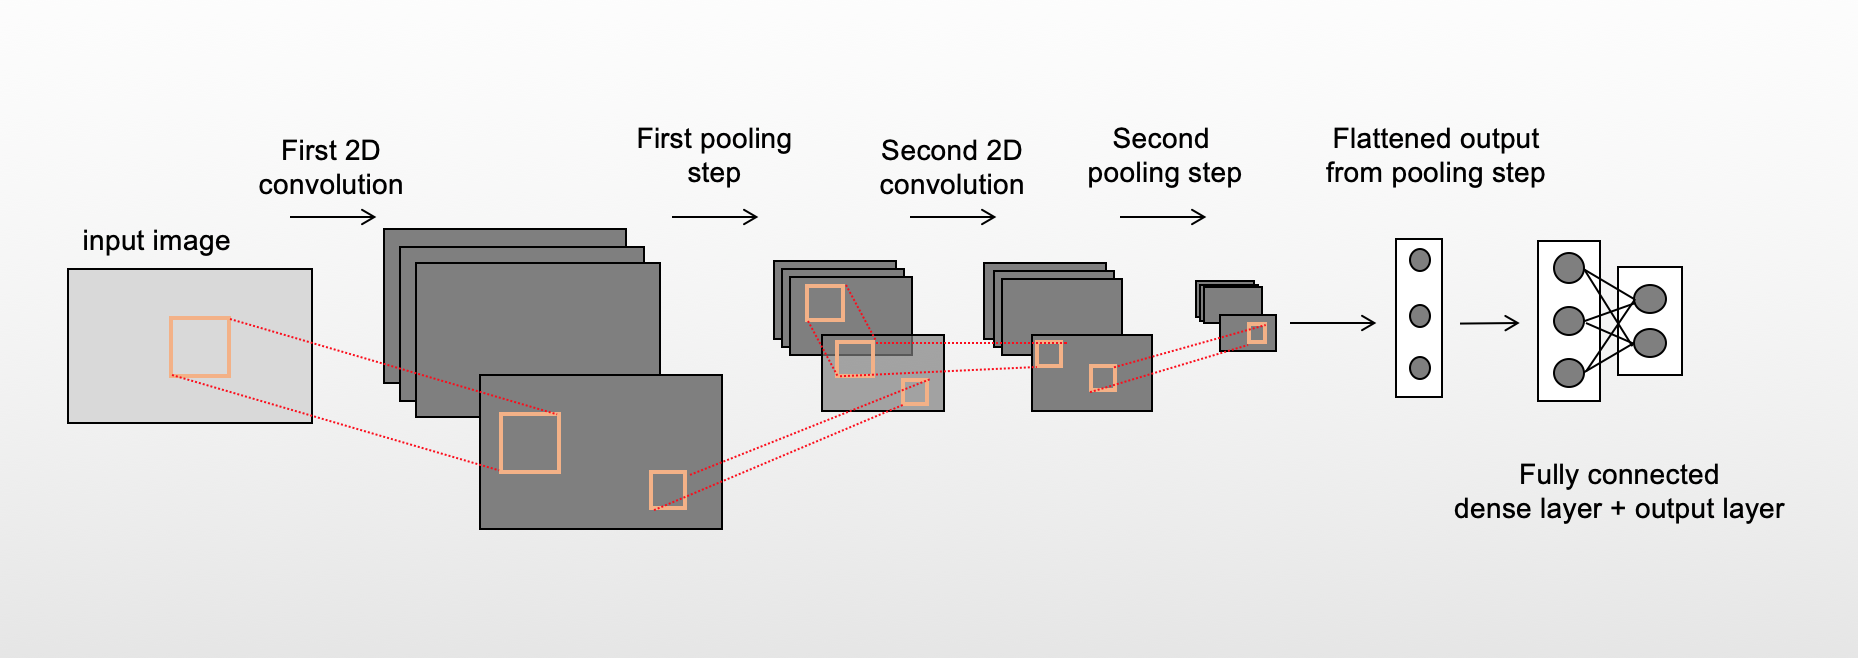
\includegraphics[trim = 0 5mm 0 5mm, clip,width=1\textwidth]{figure1.png}
  \caption{A diagram of typical 2D CNN.}
\end{figure}

\cleardoublepage\clearpage
\section{Aims}
In this study, we aim to:
\par
1. simulate genomic data for European population under categorical selection coefficients and convert it into CNN recognisable images, also explore the influence of different image representations.
\par
2. build and train CNN architectures that could quantify positive selection events and assess their properties by tuning architectures and hyperparameters.
\par
3. select CNN architectures with the best performance and test our hypothesis of possible positive selection event on \textit{NOS1AP} variant rs12143842 as well as other screened candidate variants.


\cleardoublepage\clearpage
\section{Methods}
\subsection{Target genes, negative and positive controls selection}
According to \cite{9}, there should be a reverse relationship between disease variants’ effective size and freq(1-freq) (freq stands for MAF). Therefore, in order to illustrate the unexpected high MAF of the \textit{NOS1AP} variant and screen for other candidate variants that might undergo selection event, distribution of beta estimate along freq(1-freq) for LQTS modifiers reported in two CEU-based studies \cite{4,5} can be plotted by python package plotnine \cite{26} (see Appendix 1). The target variants could then be indicated by outliners on the scatter plot.
\par
The negative control set for this study supposes to be a neutrally evolved genomic region for CEU population. Localisation of two presumably neutral regions is achieved via NRE, a tool for exploring neutral loci in the human genome \cite{27}. 
\par
The positive control we used is lactase gene variant rs4988235 G$>$A, which is a well-reckoned locus experienced distinct positive selection in CEU population \cite{28}. 
\par
With the target SNP sites in the central position, SNP information was obtained in their surrounding DNA regions (80kbp in total) via Ensembl based online-tool, Data Slicer \cite{29}. And the filter was set to CEU population. The sourcing database is 1000 genome project phase 3 with human GRCh37 assembly \cite{30}.
\par
Two summary statistics that could suggest possible positive selection event, iHS and Fay and Wu$'$s H+, are calculated to give a preliminary prediction on the two target variants and positive control. This is achieved by Haplotter (http://haplotter.uchicago.edu/) on HapMap samples of CEU population \cite{16}.
\subsection{Training data simulation }
Genomic simulator msms \cite{31} was used to simulate CEU population genomic data in this study (see Appendix 2). The demographic parameters are derived from a basic three-epoch population history model (implying a bottleneck event) suggested by \cite{32}. The mutation and recombination rate are set to 1.5e-8 and 1e-8 per bp per generation respectively, matching the typical values found in human genome \cite{33,34}. The positive selection site is set in the central and the selection time is 600 generations ago (25 years per generation). 198 haplotypes (chromosomes) are sampled in line with 99 unrelated CEU individuals in 1000 Genomes Project data. Genomic data is generated five categories of selection coefficients, 0, 0.5\%, 1\%, 1.5\% and 2\%, based on the approximate estimations of soft (0.5\%) and strong (2\%) selections in human population \cite{35,36}.
\par
100 sets of data were generated, each containing 10k replicates of genomic data for 198 haplotypes (2k replicates for each selection coefficient) (see Appendix 3). Every replicate would be converted to an image matrix using as training data for CNN later on.

\subsection{Data processing}
The core of msms output is a numeric matrix contain value 1 (alternative allele) and 0 (ancestral allele), with the rows representing haplotypes and columns representing SNP sites. However several steps required to process and prepare the initial output data for CNN training. A python-based pipeline called ImaGene (https://github.com/mfumagalli/ImaGene) was mainly employed for the data manipulation in this stage (see Appendix 4).
\par
Firstly, all major alleles (frequency $>$ 0.5 among 198 haplotypyes) were coded as value 1 and minor alleles as value 0 to account for the inconsistence of ancestral allele annotation between simulated data and real data. Minor alleles that have frequency lower than 0.01 were also removed to reduce the noise of images. 
\par
Based on previous CNN training researches, reordering rows (haplotypes) in genomic images can help CNN training better learn the features of selection signatures \cite{17}. The default sorting option provided in ImaGene is by their frequency of occurrence. Here in this study we also managed to implement a genetic distance sorting method inspired by \cite{17}$'$s study into ImaGene and apply both sorting options to our data. The new sorting method take advantage of the neighbors function in scikit-learn package \cite{44} in python to cluster the haplotypes based on their genetic similarity. 
\par
Moreover, sorting the columns in the same way seems not to affect CNN training accuracy meanwhile allow a less weighted CNN architecture . Therefore,we kept the option of double-sorting (both rows and columns) for our data.
\par
Lastly, the whole matrix was then resized to 198x198 pixels.

\subsection{CNN architecture building}
The CNN models build in this study used two python packages, Keras \cite{37} doing high-level building and training of network layers and TensorFlow \cite{38} working as backend that does underlying calculations.
\par
We begin with binary classifier and then proceed to multiple categories classifier (see Appendix 5 \& 6). The binary classifier predicts two possible labels, and we tried for two sets (0, 1.5\%) and (0, 1\%). The categorical classifier takes all five labels.
\par
For binary classifier in our study, the default configuration was set to be 3 max pooling layers on top of three convolutional layers, linking to 1 dense layer. The filter number was given 32 and size (3x3) as a default setting \cite{39}. The activation function, which applies non-linearity to the output value, was given ReLu for both convolutional layer and dense layer, and sigmoid for output layer. The loss function and optimizer, which monitor the training performance and guide back-propagation that tunes the CNN parameters, used rmsprop and binary\_crossentropy respectively.
\par
For the categorical classifier, the default configuration was same as that for the binary. Only activation function for output layer changed to softmax and the optimizer changed to categorical\_crossentropy.

\subsection{Model training and hypertuning}
CNN training is computationally intensive. The categorical trainings were operated on cloud-based GPU and the binary trainings were operated on local CPU (see Appendix 5 \& 6).
\par
Images/matrixes in each training image set were randomly shuffled around. 1/10 of them were held for validation in each epoch of training to monitor the loss and accuracy, which was later plotted to indicate the training process. 
\par
Among all the employed data sets, one entire set was left as test set to test the accuracy of the whole training process and enabled the confusion matrix plotting (a table for visualising accuracy in multi-class classification).
\par
Extensive model trainings have been run with a large range of hyperparameters being tested. The hyperparameters tuning includes number of training data sets (50 sets as default), numbers of training epoch (rounds for training through the same training data set) (one as default), number of filters in convolutional layer (32 as default), number of convolutional layers (three as default) and with or without dense layer. These variables all account for the parameter number and total efficacy of the training model.
\par
In general, CNN trainings were performed for both images sorting options in two binary classifiers and one multiple categorical classifier, with the hyperparameters varying from ran to ran.


\subsection{Model selection and target variants prediction}
In all three classifiers, one best model was chosen based on accuracy and efficacy.
\par
Target genomic data that obtained by Data Slicer and stored in VCF files were extracted by Python package scikit-allel \cite{45} and restored into Python numpy arrays (see Appendix 7). The following processes for data were achieved in Python  and kept consistent with that of the simulation data. Finally, the chosen trained algorithms were used to predict the selection coefficient class for genomic data converted from target variants (see Appendix 8).



\cleardoublepage\clearpage
\section{Results}
\subsection{Target variants, positive and negative control}


The distributions of beta estimate along freq(1-freq) for both studies are plotted in Figure 2. \textit{NOS1AP} variant rs12029454 together with rs12143842 were picked as outliners basing on two graphs, and they are likely to be targets of positive selection event. In addition, rs12143842 is located upstream \textit{NOS1AP} while rs12029454 is in intron region of \textit{NOS1AP}, and they are individual signals detected with QT interval association \cite{4,5}.

\begin{figure}[H] 
  \captionsetup{singlelinecheck = false, justification=justified}
  \centering
  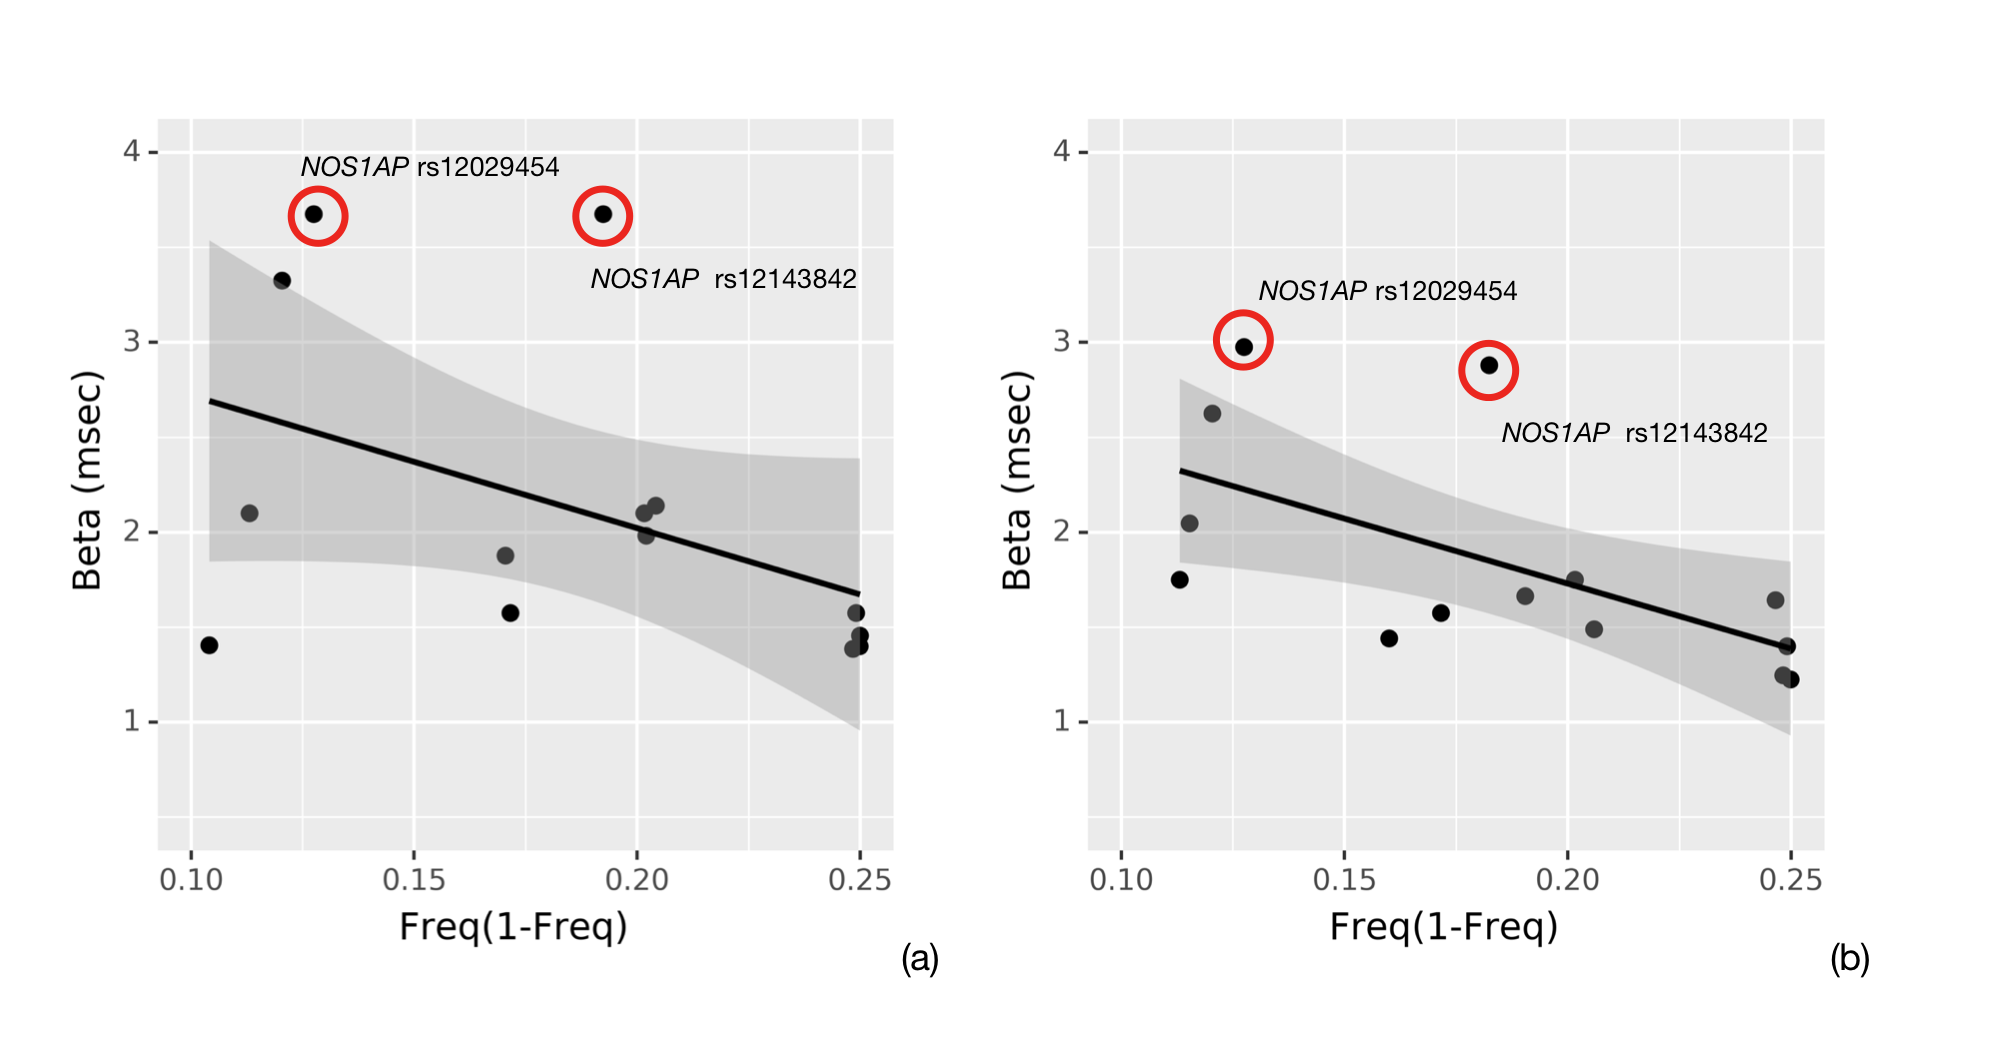
\includegraphics[trim = 0 5mm 0 5mm, clip,width=1\textwidth]{figure2.png}
  \caption{Distribution of beta estimate (msec) along freq(1-freq) for same set of variants in (a) QTGEN study and (b) QTSCD Study. The regression lines and margins indicate the reverse relationships. Red circles annotate the outliners.}
\end{figure}

Preliminary prediction on two target variants and positive control variant using summary statistics (iHS, Fay and Wu$'$s H+) is listed below (Table 1), indicating a possible positive selection event acting on our target variants.

\begin{figure}[H] 
  \captionsetup{singlelinecheck = false, justification=justified}
  \centering
  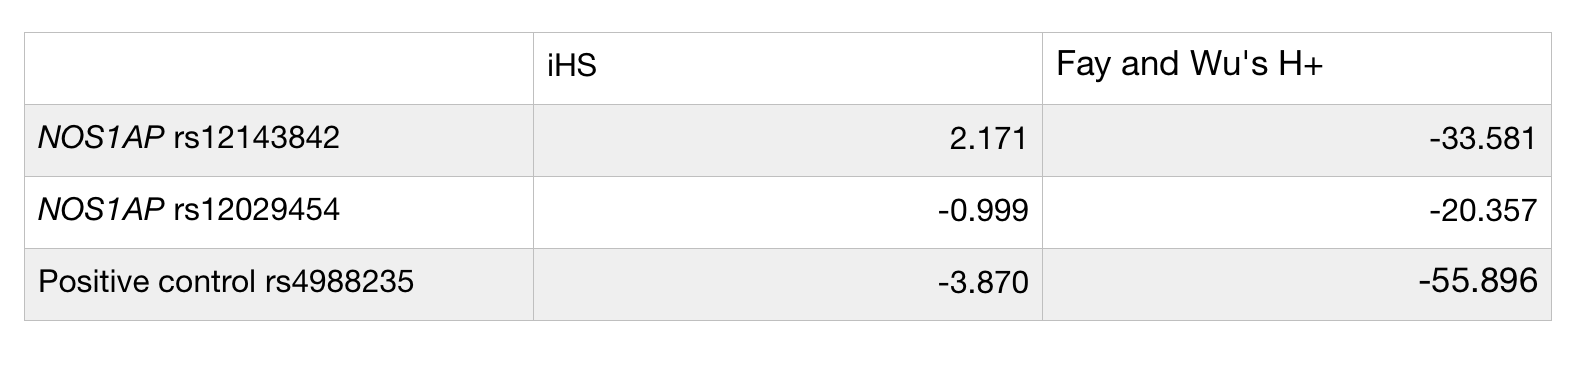
\includegraphics[trim = 0 5mm 0 5mm, clip,width=1\textwidth]{table1.png}
  \captionof{table}{Large negative value of Fay and Wu$'$ H+ and |iHS| $>$ 2 indicate selection events.}
\end{figure}

Information of genomic segments obtained for two target variants and three control variants is summarised in Table 2.

\begin{figure}[H] 
  \captionsetup{singlelinecheck = false, justification=justified}
  \centering
  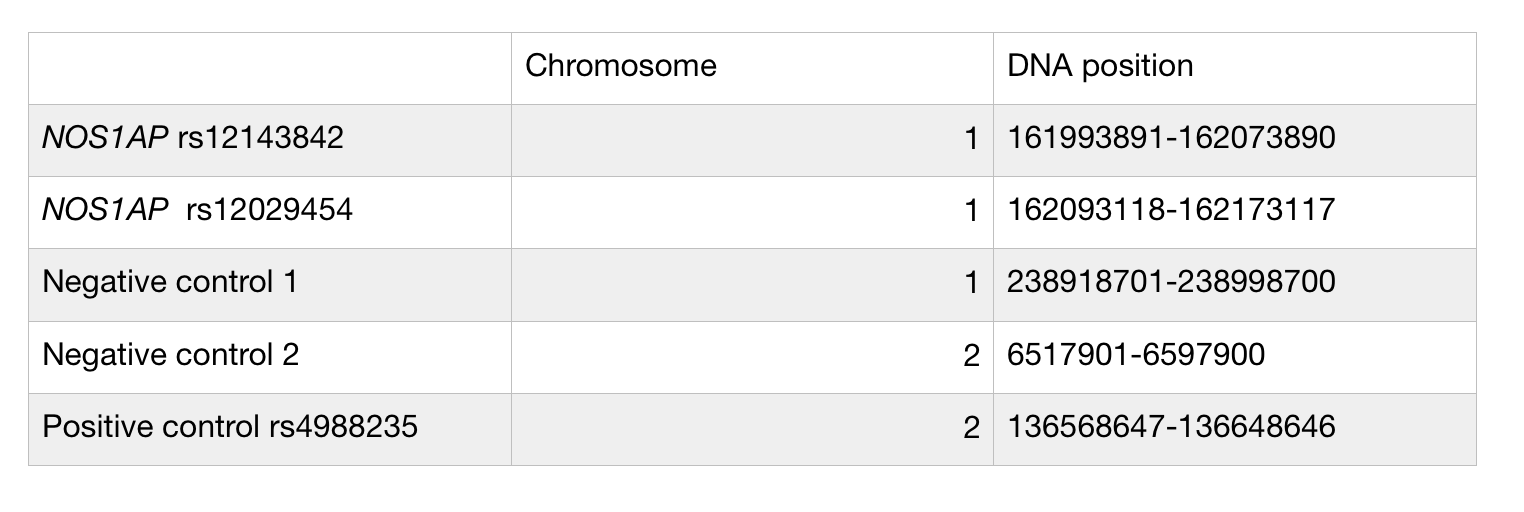
\includegraphics[trim = 0 5mm 0 5mm, clip,width=1\textwidth]{table2.png}
  \captionof{table}{Genomic segments for target variants and control variants.}
\end{figure}

\subsection{Simulation and data presenting}
The simulated data is stored in 100 folders, each is a data set containing 10k simulated matrixes/images for 5 classes of selection coefficients in total. 
\par
Visualisation of matrixes simulated under different selection coefficients is shown is Figure 4 below. These are examples from the simulation pool. Figure 3 and 4 present images that were double-sorted by frequency of occurrence and genetic similarity, respectively. 
\begin{figure}[H] 
  \captionsetup{singlelinecheck = false, justification=justified}
  \centering
  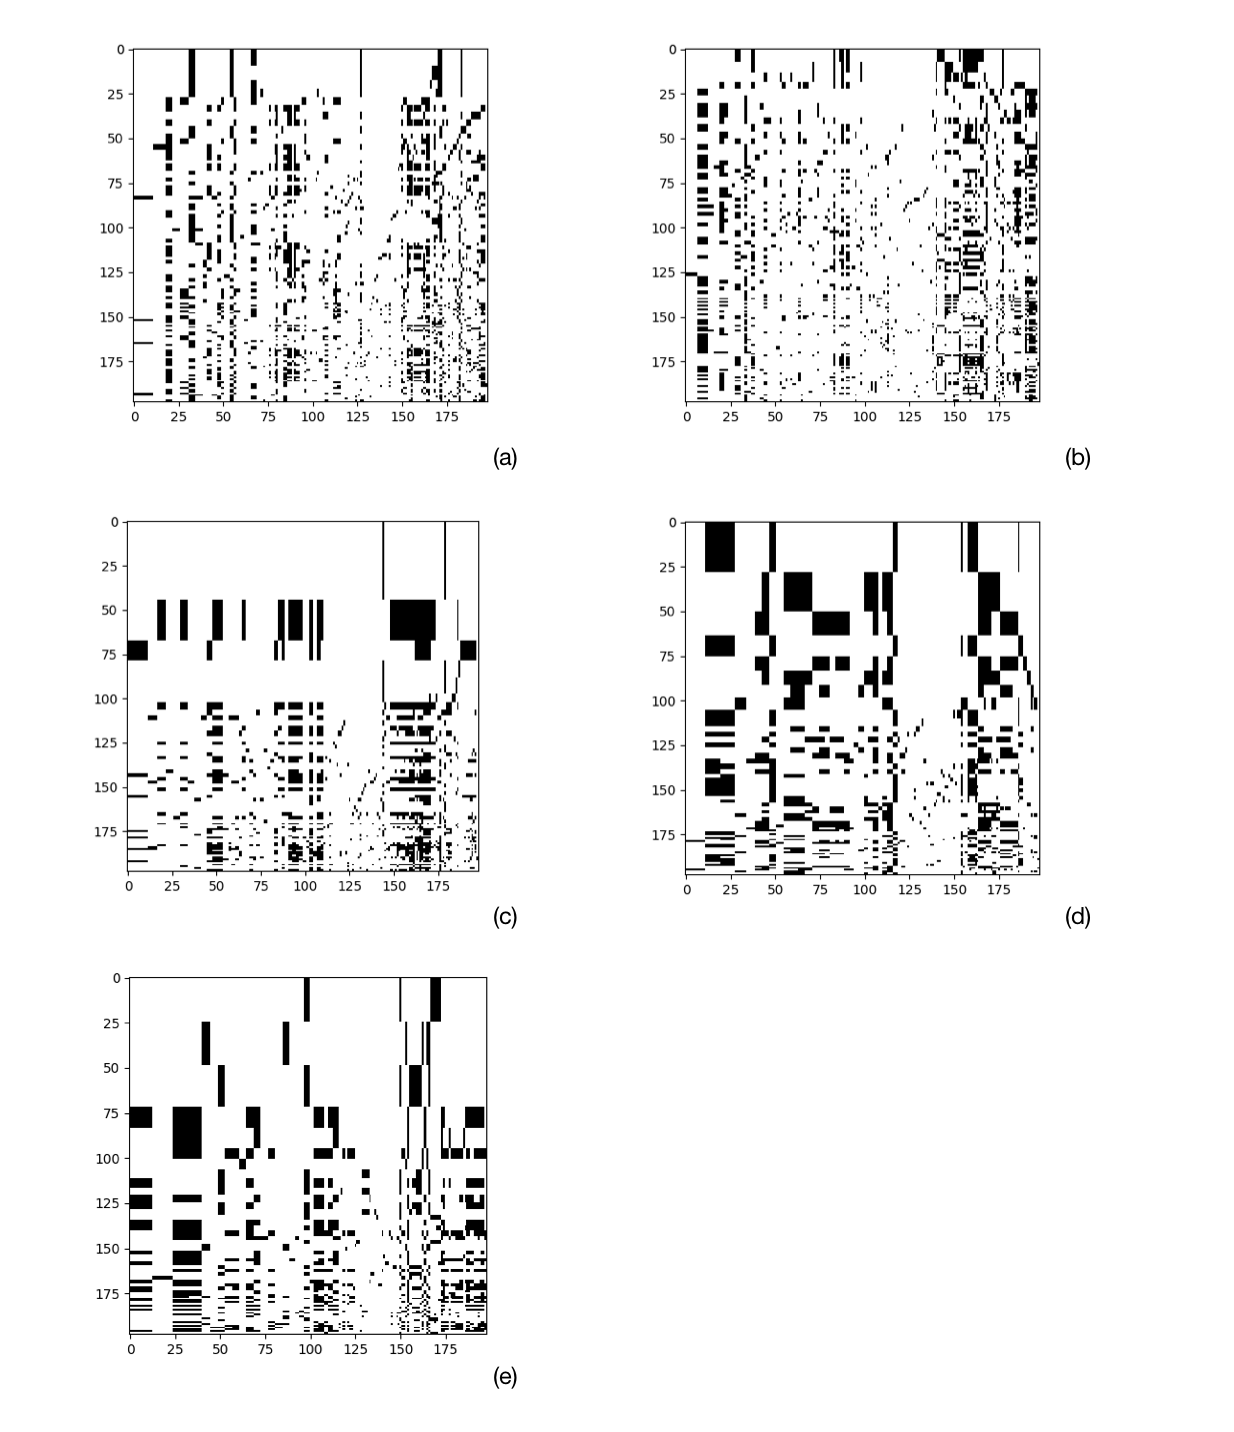
\includegraphics[trim = 0 5mm 0 5mm, clip,width=1\textwidth]{figure3.png}
  \caption{Images sorted by frequency in both row and columns. (a) - (e) shows 5 selection scenarios with coefficients ranging from 0 to 2\%.}
\end{figure}

\begin{figure}[H] 
  \captionsetup{singlelinecheck = false, justification=justified}
  \centering
  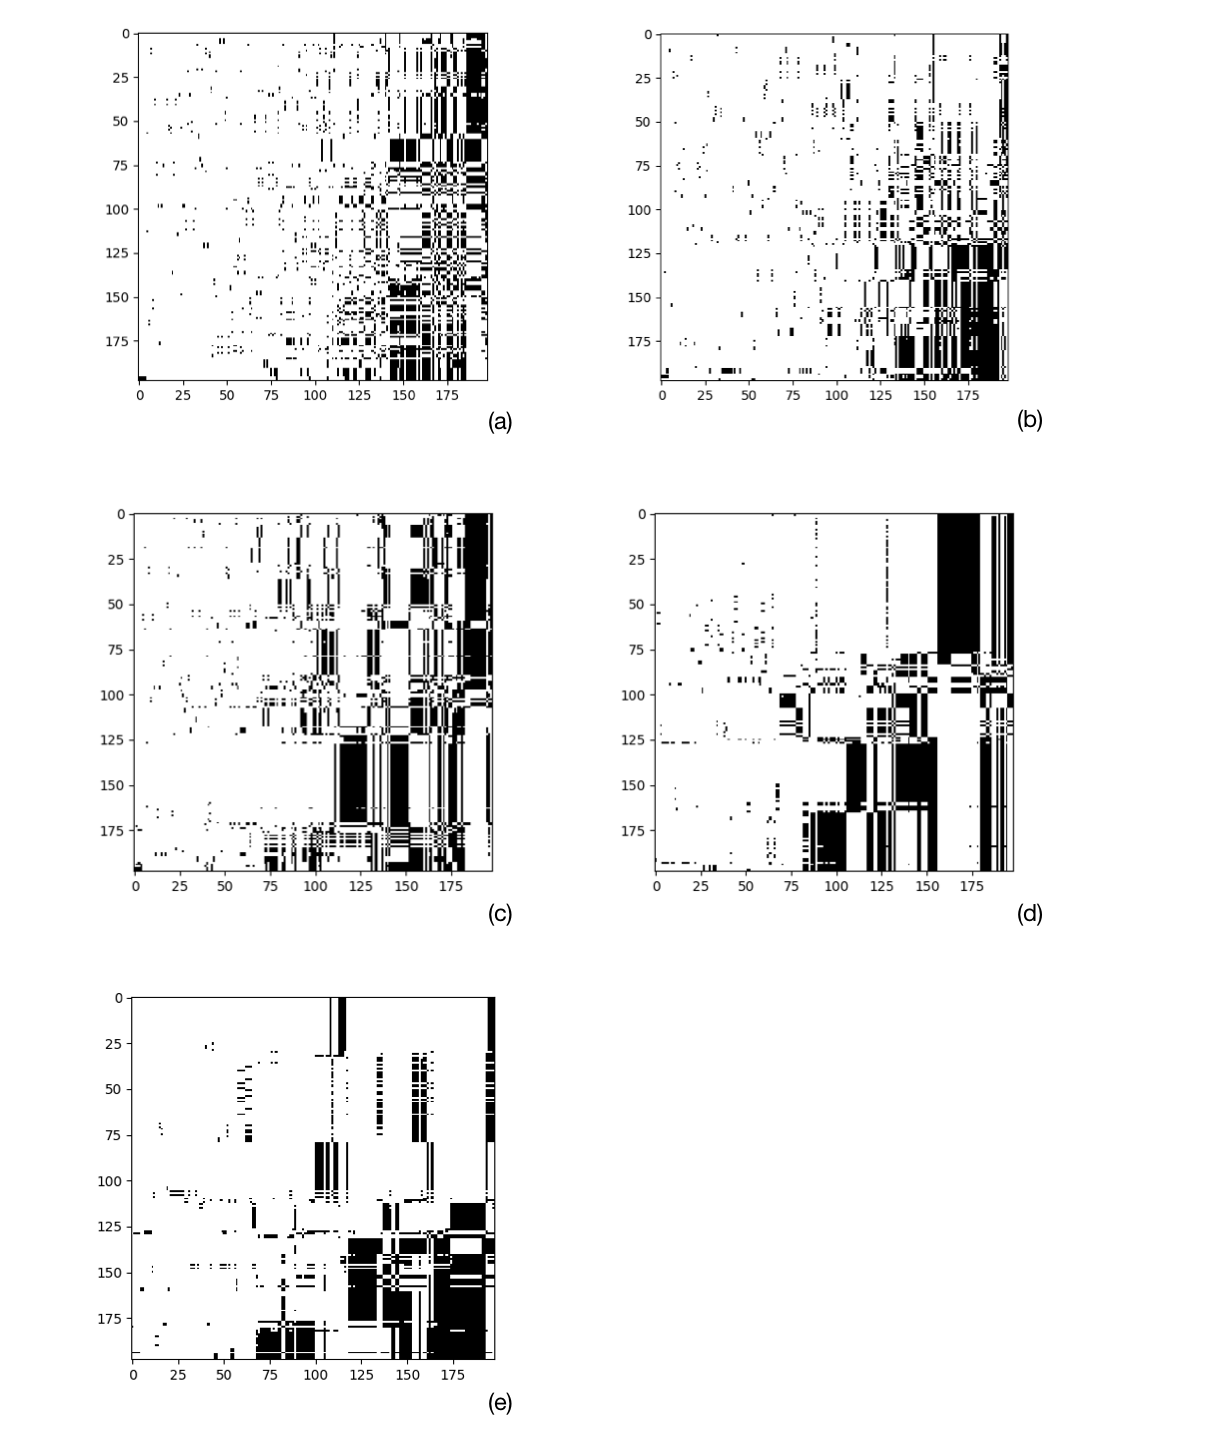
\includegraphics[trim = 0 5mm 0 5mm, clip,width=1\textwidth]{figure4.png}
  \caption{Images sorted by genetic similarity in both row and columns. (a) - (e) shows 5 selection scenarios with coefficients ranging from 0 to 2\%.}
\end{figure}

For both sorting options, the image pattern changes along selection coefficients. The black blocks are quite scattered in the image when selection coefficient is low (for example 0 or 0.5\%). On the other hand, they become more and more clustered when selection coefficient rises to 1.5\% or 2\%.

\subsection{Trained CNN models}
The test runnings show that, for both sorting options, accuracy of models (default configurations for binary classifiers and the categorical classifier) does not seem to vary between double sorting approach and row sorting alone. Therefore, double sorting is used in image presenting for CNN models in our study.
\par
For the binary classifiers, CNN configuration of more than four convolutional layers seems to cause failure in the learning process of CNN model resulting in low accuracy close to random guessing. CNN learning failure can be seen from the confusion matrix and the training and validation loss and accuracy (TVLA) graph (Figure 5) 
\begin{figure}[H] 
  \captionsetup{singlelinecheck = false, justification=justified}
  \centering
  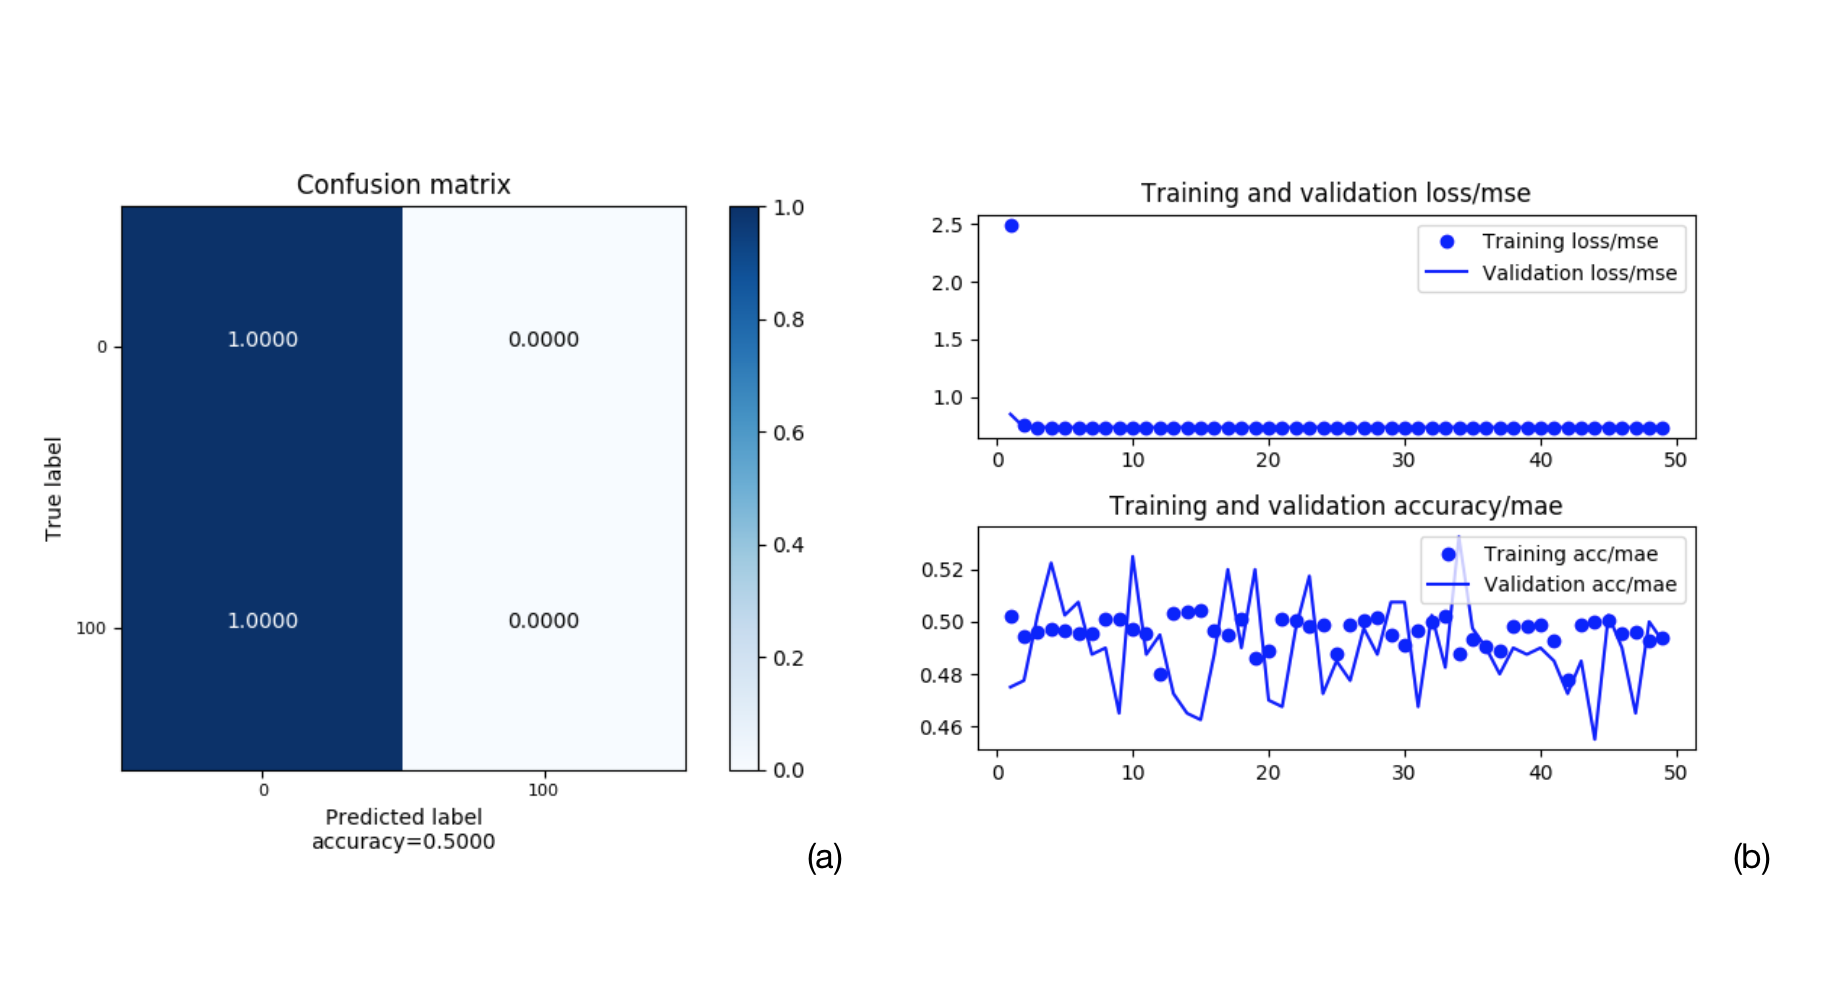
\includegraphics[trim = 0 5mm 0 5mm, clip,width=1\textwidth]{figure5.png}
  \caption{An example of CNN learning failure. The confusion matrix (a) shows an accuracy of 50\%. In TVLA graph (b), as the training process carries on for more data sets, the loss did not gradually reduce and neither did accuracy increase as expected.}
\end{figure}

Meanwhile, increasing the convolutional layers from three to four solely does not improve the accuracy of binary classifiers. Therefore three convolutional layers are set as default. For the other hyperparameters, CNN model training results for two binary classifiers and two sorting options are summarised in Table 3 \& 4. 

\begin{figure}[H] 
  \captionsetup{singlelinecheck = false, justification=justified}
  \centering
  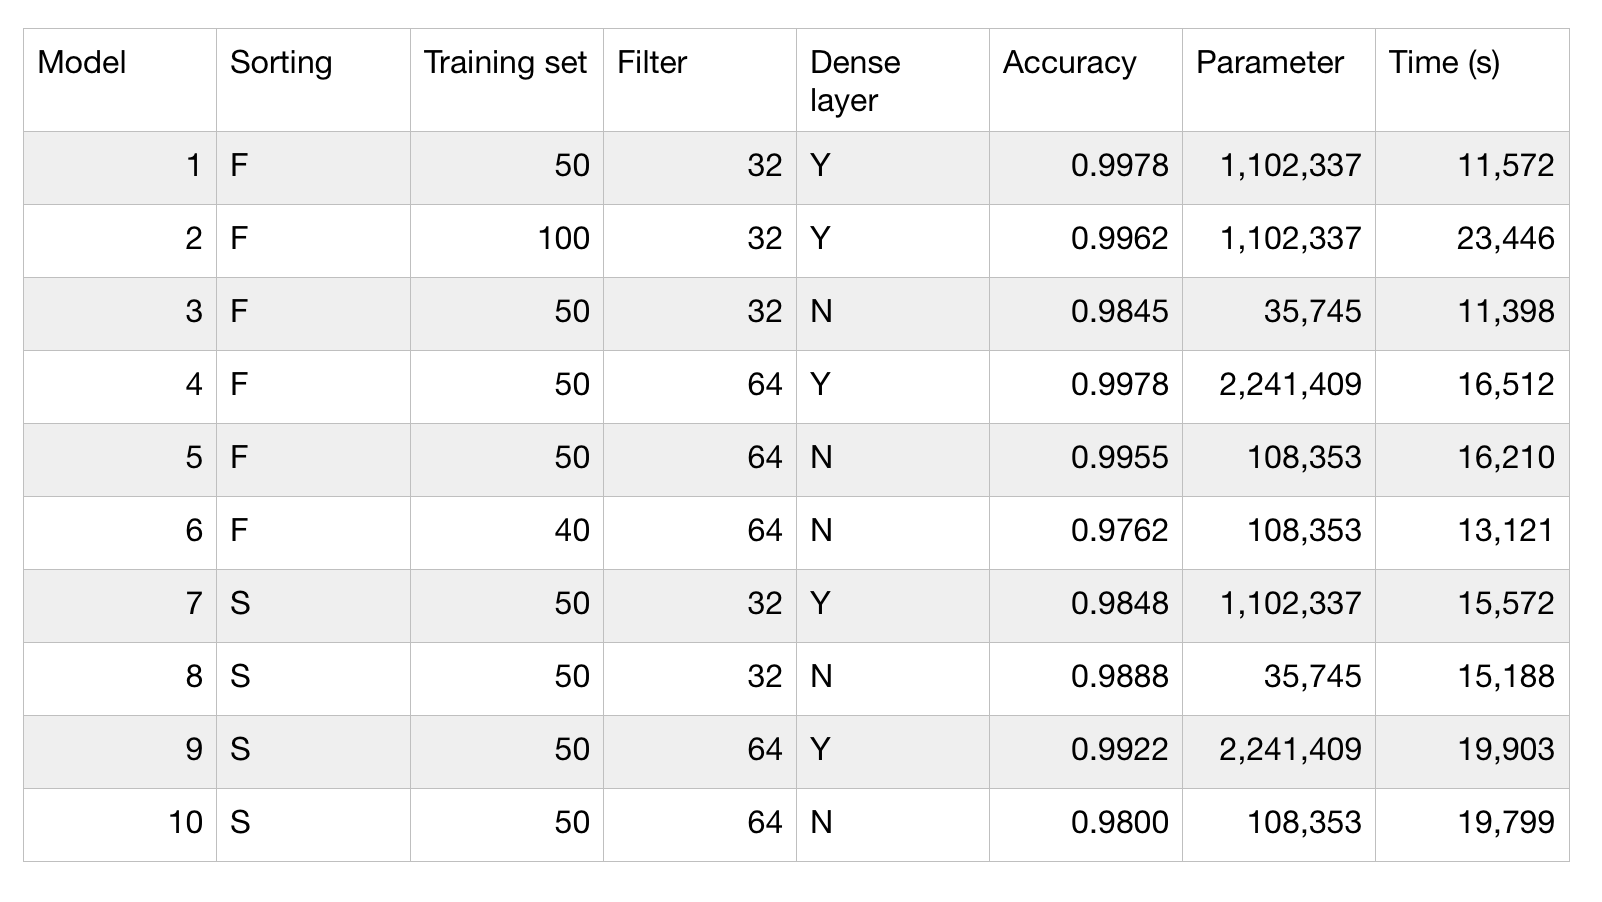
\includegraphics[trim = 0 5mm 0 5mm, clip,width=1\textwidth]{table3.png}
  \captionof{table}{CNN model trainings for binary classifier [0, 1.5\%]. In sorting column, F stands for frequency, S stands for genetic similarity.}
\end{figure}

\begin{figure}[H] 
  \captionsetup{singlelinecheck = false, justification=justified}
  \centering
  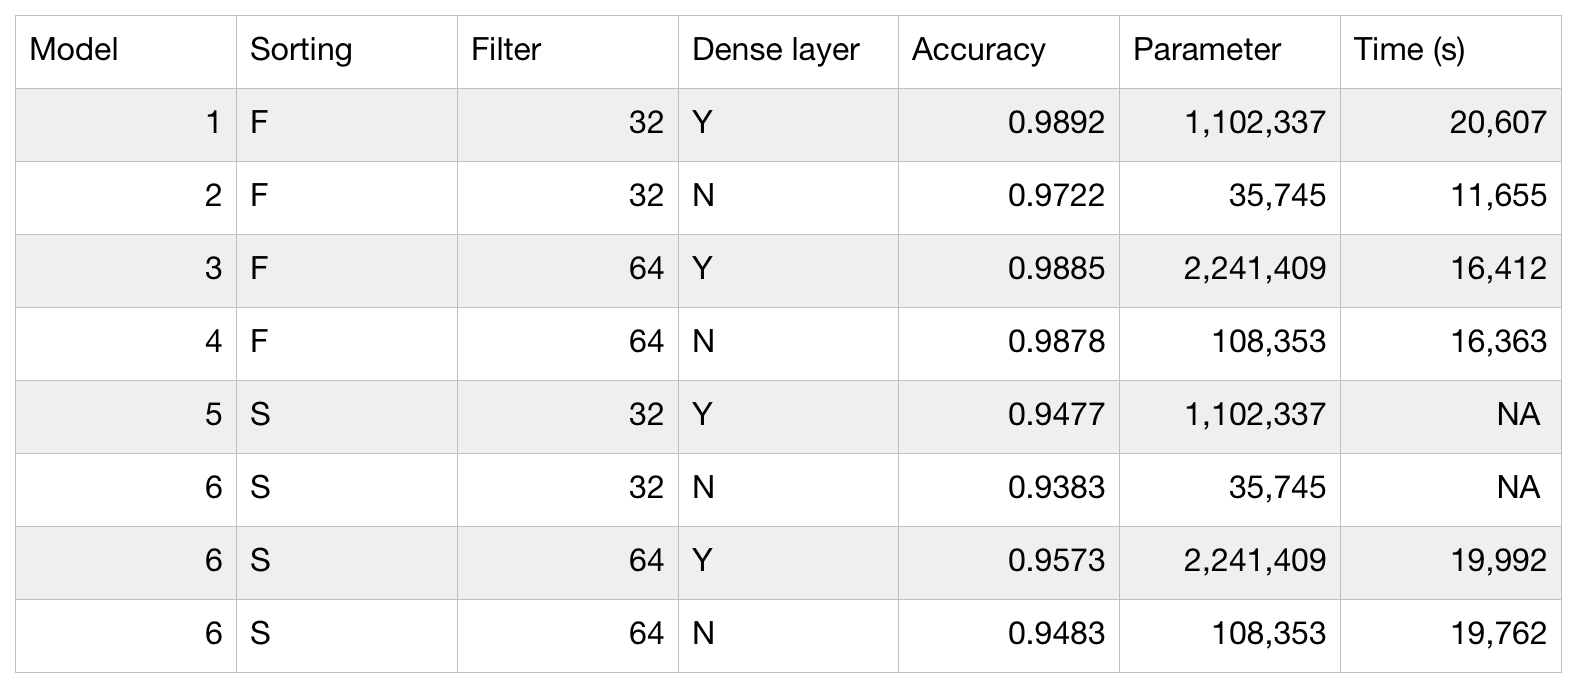
\includegraphics[trim = 0 5mm 0 5mm, clip,width=1\textwidth]{table4.png}
  \captionof{table}{CNN model trainings for binary classifier [0, 1\%]. In sorting column, F stands for frequency, S stands for genetic similarity.}
\end{figure}


We also carried on with finer classification by training CNN model to [0, 0.5\%] labels. However, the CNN learning process failed and the accuracy dropped to 50\% which is same as random guessing.  
\par
For the categorical classifier, convolutional layers more than three leads to unsuccessful training. Hence, the number of convolutional and max pooling layer pack is set to three. While the other hyperparameters tested in CNN models for two sorting options are summarised in the table below (Table 5).

\begin{figure}[H] 
  \captionsetup{singlelinecheck = false, justification=justified}
  \centering
  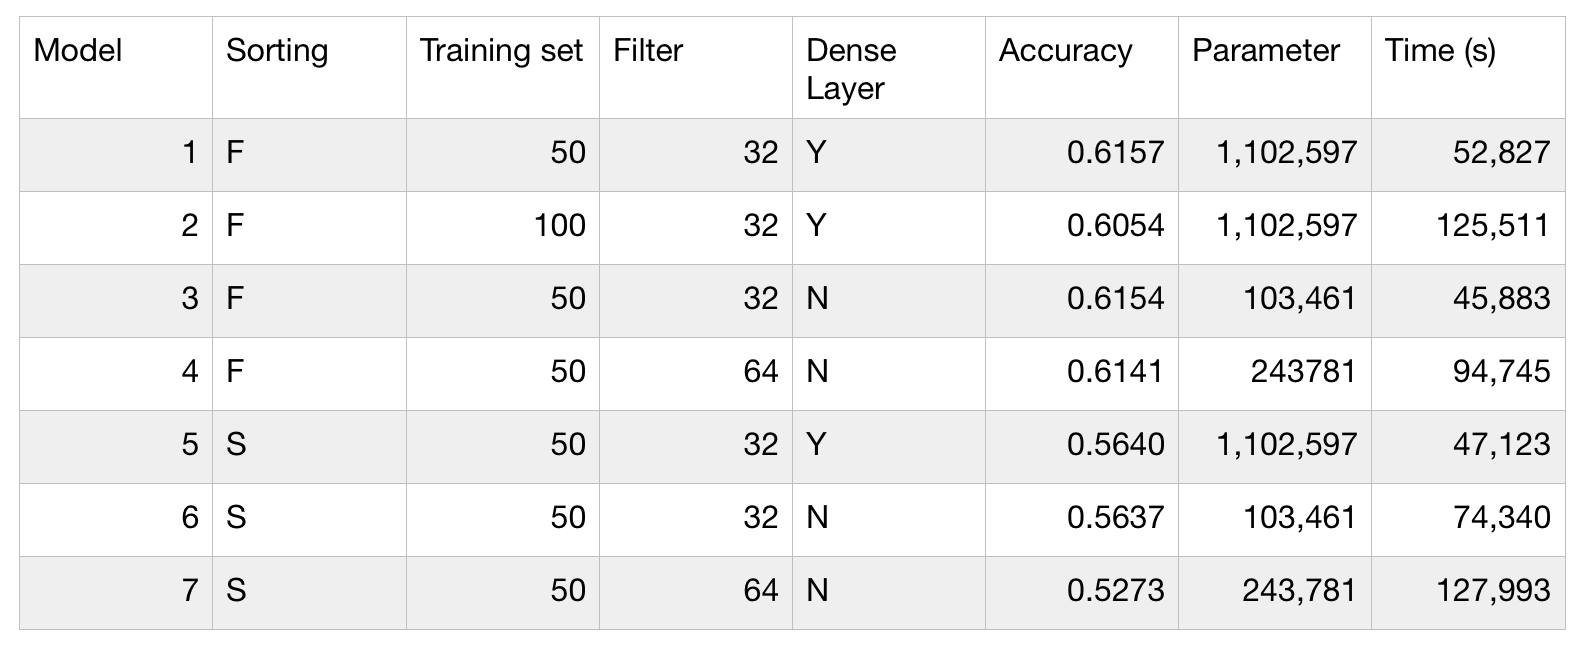
\includegraphics[trim = 0 5mm 0 5mm, clip,width=1\textwidth]{table5.png}
  \captionof{table}{CNN model trainings for categorical classifier [0, 0.5\%, 1\%, 1.5\%, 2\%]. In sorting column, F stands for frequency, S stands for genetic similarity.}
\end{figure}


In general, CNN models trained by images of frequency sorting perform better than that of genetic similarity based sorting. Besides, it is difficult for the algorithms to distinguish between closely ranked labels. Removing the dense layer might slightly impair the accuracy however largely reduce the model parameters needed. Increasing training data sets or convolutional filters can have minor or no improvement on accuracy especially for categorical classifiers. Meanwhile they significantly increased the training time required. 
 
 
\subsection{Model selection and variants prediction}
Based on the accuracy and model complexity, models that have 64 filters, no dense layer and images sorted by frequency are chosen for binary classifiers, and the categorical classifier is given the model with 32 filters without dense layer and frequency sorting images. Their confusion matrixes and TVLA graphs are showed below (Figure 6).

\begin{figure}[H] 
  \captionsetup{singlelinecheck = false, justification=justified}
  \centering
  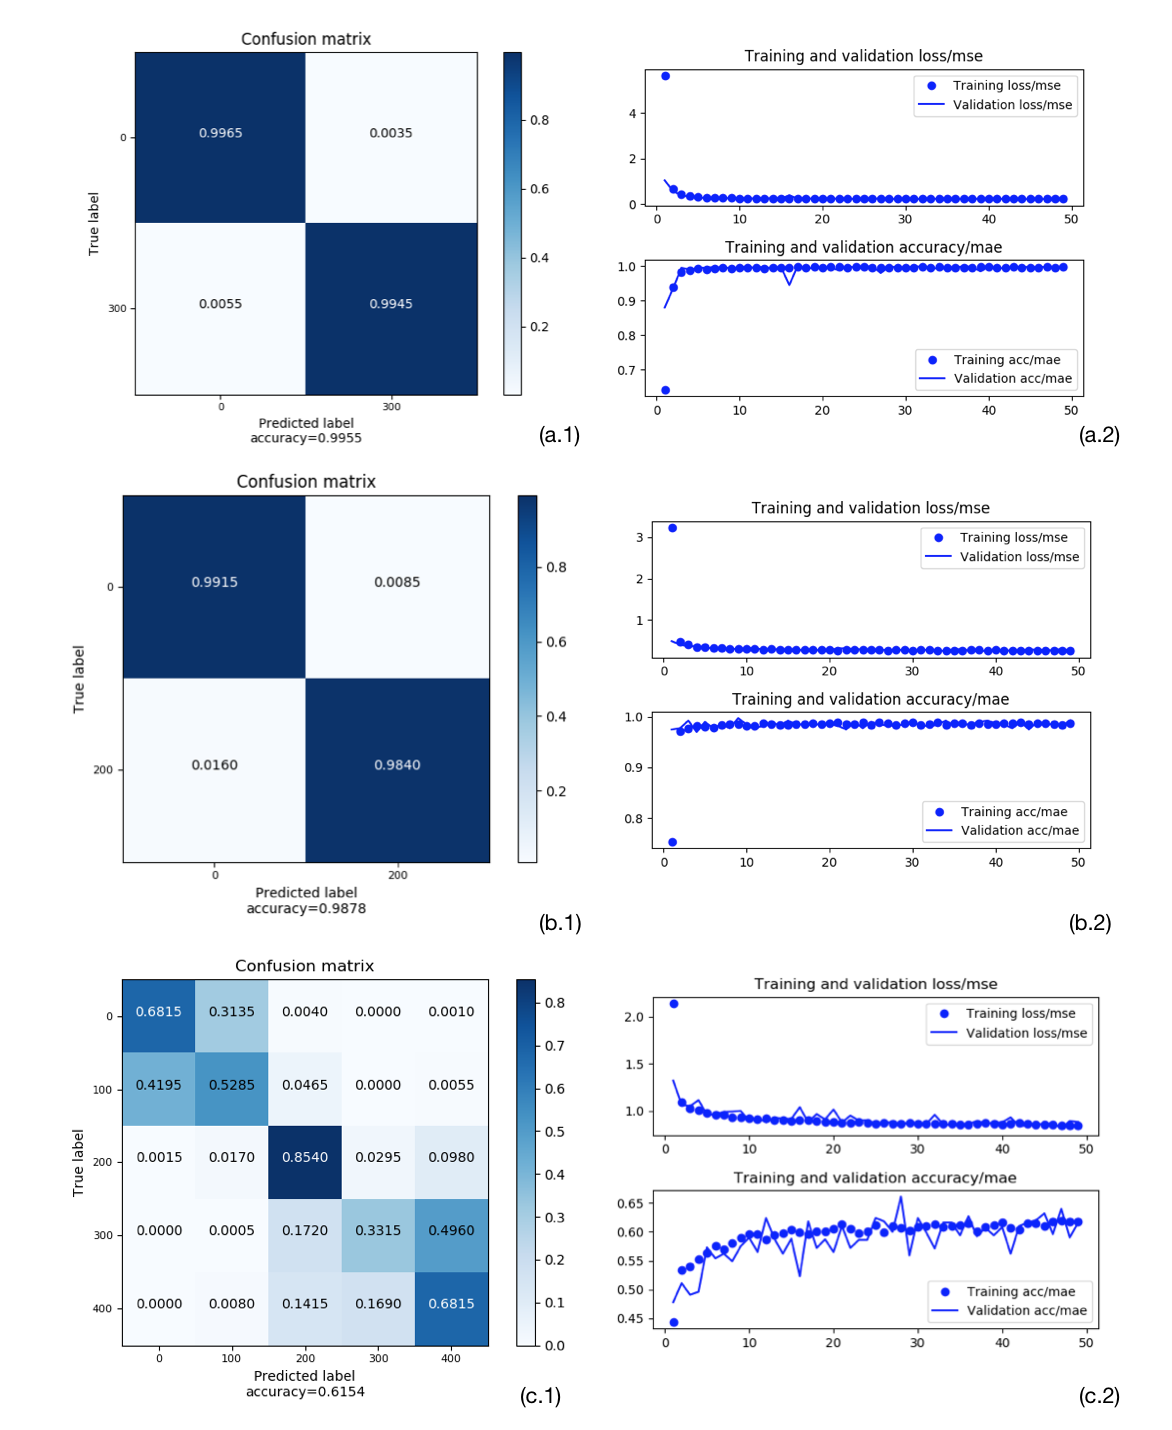
\includegraphics[trim = 0 5mm 0 5mm, clip,width=1\textwidth]{figure6.png}
  \caption{Column (a) is confusion matrix and (b) is TVLA graph. Row (1) is for categorical classifier, row (2) is for binary classifier [0, 0.5\%], row (3) is for binary classifier [0, 1\%].
}
\end{figure}

The prediction results for positive and negative control variants as well as two targeted variants are listed below (Table 6). These results seem not to support our hypothesis of positive selection on two \textit{NOS1AP} variants.

\begin{figure}[H] 
  \captionsetup{singlelinecheck = false, justification=justified}
  \centering
  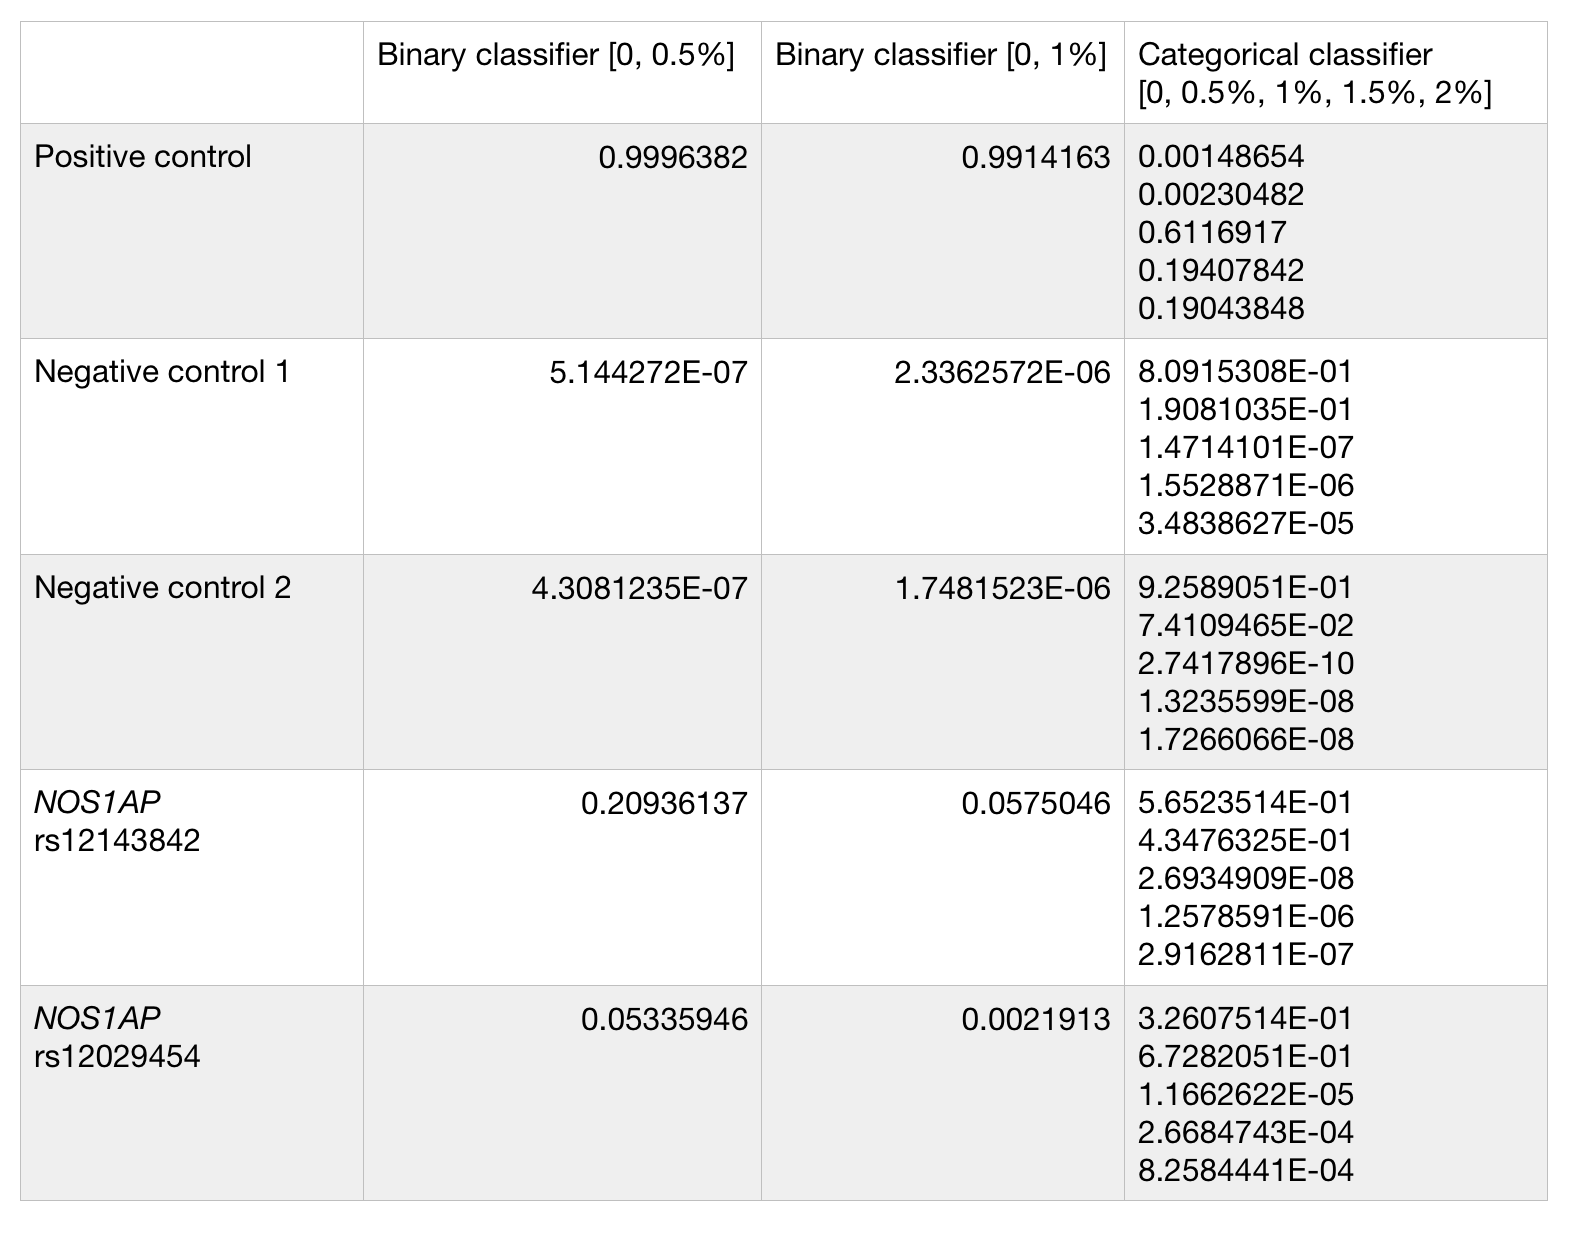
\includegraphics[trim = 0 5mm 0 5mm, clip,width=1\textwidth]{table6.png}
  \captionof{table}{For binary classifier, the values are possibility of belonging to the upper rank. For categorical classifier, the values are possibility of belonging to the corresponding ranks.}
\end{figure}

Interestingly, although models trained with images of genetic similarity sorting have a slightly low accuracy and are therefore not selected for target variants prediction, their predictions on negative control seem to suggest a positive selection event, which is unexpected.

\cleardoublepage\clearpage
\section{Discussion}

\subsection{Evaluation on model training and prediction}

During this study, we have successfully simulated genomic segments containing SNPs information for pre-defined population history and selection events. The images converted from genome simulator have distinct patterns representing different selection scenarios. We have also built and trained a range of CNN models that could distinguish those grouped images by learning their patterns. 
\par
By evaluation on both model hyper-tuning and image representing, we observed that CNN models trained by images of frequency sorting can generally achieve higher accuracy meanwhile consume less training time, compared to that of genetic similarity based sorting in a range of environments. We were also surprised to see that increasing training data sets from 50 to 100 or adding convolutional filters from 32 to 64 all presented quite limited effect on accuracy improvement expected for categorical classifiers or classification on closer binary labels.
\par
Interestingly, dropping the dense layer might not impair the model accuracy, when the training images are sorting for both rows and columns. For binary classifiers, removing the dense layer could decrease the accuracy for around 0.01. Meanwhile for categorical classifier, more subtle influence was observed. However for all models, running without dense layer reduce the total parameters needed in CNN model by more than 95\%. Although reduced parameter does not necessarily lead to less training time, it generates a less-weighted model which have fewer inner functions involved (less prone to errors) meanwhile achieving the same output. 

\par
Nevertheless, raising filter from 32 to 64 can slightly improve the accuracy by 0.01 for binary classifiers without dense layer. Therefore we suggest that “64 filters with dense layer” configuration is preferred in binary classifier and “32 filters without dense layer” is better used in categorical classifier. The image sorting option was kept for frequency sorting.

\par
Although predicting labels between selection coefficient 0 and 0.5\% is more difficult than that for 0 and 1\%, both classifiers perform a decent accuracy. Our finial classifier [0, 0.5\%] has an accuracy of 0.9955, while classifier [0, 1\%] has 0.9878.
\par
Compared to binary classifiers, the categorical classifier is less accurate. The final model we employed shows an accuracy of 0.6154. However, if we give a closer look at the confusion matrix of this model (Figure.8), we can find that it generally fails at distinguishing between 0 and 0.5\% or 1.5\% and 2\%, meanwhile able to differentiate no selection (0 and 0.5\%), moderate selection (1\%) and strong selection (1.5\% and 2\%). Therefore we could reallocate our categorical classifier result into three labels instead of five, which means their accuracy would be up-graded to round 95\% for distinguishing between three levels of selection. 
\par
The predictions on negative controls all indicate them to be evolved under neutrality, which meet our expectation. And the prediction on lactase variant, the positive control, suggests it has experienced at least a moderate positive selection (selection coefficient 1\%, 600 generation). However, all three classifiers fail to suggest significant positive selection events happened on the two target variants.
\par
Compared to the results for two negative controls, which indicate great possibilities of them failing in 0 selection coefficient category, prediction for both \textit{NOS1AP} variants leaves a margin for weak positive selection. Because both the binary classifiers show a much larger value compared to 5e-07. And since the categorical classifiers fail to distinguish between 0 and 0.5\% positive selection scenarios, we can only conclude that there is a high possibility (more than 99\%) that \textit{NOS1AP} variants should not experience positive selection that has selection coefficient of 1\%,1.5\% or 2\% (600 generations). 
\par
Therefore, we cannot rule out the possibility of weak positive selection around 0.5\% for \textit{NOS1AP} variants. One possible scenario is that these variants might undergo positive selection in the past in European populations. Lately, and very recently, this variant became unfavored due to environment or lifestyle shifts. Additionally, the pleiotropy effect of gene (one gene effects more than one phenotypic trait) might also explain the soft positive selection event of these disease modifier variants. In fact, it was suggested that variants conferring to cardiac repolarisation could also affect other tissues or contribute to early stage development, and can therefore be maintained in the population via selection \cite{10}. 
\par
In general, we are confident to suggest that both \textit{NOS1AP} variants rs12143842 and rs12029454 have not been through significant positive selection. However they might not evolve under complete neutrality. It is more likely that they experienced soft selection event of selection coefficient around 0.5\% (600 generations).  
\par
It is difficult to compare this prediction result with that of other positive selection detection methods, such as the two summary statistics we used for preliminary prediction, iHS as well as Fay and Wu$'$ H+ because these methods do not quantify the selection event. Even their evaluation for the strength of selection is in different measurement system. Therefore direct comparison between the detection results on single variant is not feasible. However, when we carry out comparison between three variants (two \textit{NOS1AP} variants and the positive control variant), the results are consistent across different methods. All predictions suggest that \textit{NOS1AP} variants might have experienced some extent of selection however much weaker than that acted on positive control variant rs4988235.

\subsection{Influence of image presentation on CNN classifier}
\par
One notable question remained in the whole study is that two negative controls are predicted to be positively selected by CNN models trained with images of genetic similarity based sorting. This is unexpected since these models were trained same as those have frequency sorting images and the training processes went smoothly. Although they have slightly lower accuracy, the binary classifiers can still reach to about 99\% accuracy.
\par
One possible explanation for this inconsistent result is that the sorting option might have systematic bias in presenting the pattern features. It is possible that this sorting approach has somehow weakened the robustness of CNN model on the pre-assumptions, such as demographic history and selection scenario. Since the training data are generated basing on those pre-defined assumptions, when the assumptions are not close enough to the reality or the model is sensitive to the assumption deviation from the reality, the trained algorithm would be tested on new data not belonging to any training data groups. Therefore unexpected prediction would be witnessed, as the features that CNN model learnt became useless when it faces different types of data that it has not been trained to learn. 



\subsection{Limitations and future work}
Although we tried to preserve relatively complete genomic information in images/matrixes, the images used in this study did not inherit entirely from the simulated genomic segments or segments of real genome. The columns which contain no polymorphisms among the 198 haplotypes were removed to highlight the clustered patterns. Because the majority of the columns are blank (no polymorphisms), including them might conceal the informative features. However removing the blank columns also lose part of the genomic information, which is the relative position of SNPs along the genomic region. For the classifier algorithm, losing information means less to learn and therefore accuracy reduces. 
\par
It is suggested that one way to improve this situation is by introducing a 1D CNN model learning the position information pairwise to our current 2D CNN model \cite{17}. (1D CNN means the input is in 1D array and 2D CNN means the input is 2D image.) The two CNNs can then be concatenated before the output layer. In this way, more complete genomic information from genome is designed to be learnt by the classifier algorithm. Although in reality, technique problems should exist for successfully training that complex model to learn the desired features and produce satisfactory accuracy.
\par
A second drawback is that we had only one demographic model tested. As mentioned above, if the pre-assumptions are closer to reality, the training data would enable model algorithm to learn more accurate features that can be used to analyse the real data. Hence, depending on the robustness, better model assumption could correct the prediction or at least increase the accuracy of the model. Although we were expecting some extent of robustness in our classifiers on one basic demographic background, more demographic models are in need to test its sensitivity and hopefully improve the accuracy. There are currently a few complex demographic models proposed for CEU population \cite{42,43}. These models include population migrations, varying recombination and mutation rates and more detailed timeline of bottleneck events, which should better resemble the realistic population history. 
\par
Theoretically, using simulated data with pre-defined selection coefficients to train a CNN model could enable the quantification of selection events, as along as the trained algorithm shows desired accuracy. However currently, our categorical classifier has only about 60\% accuracy for 5 labels. If we need at least 90\% confidence we have to reduce five labels to three, which means the we can only roughly quantify the selection coefficient to three ranks (0 or 0.5\%; 1\%; 1.5\% or 2\%). Although the paradigm of image based CNN classifier for genetic inference, reported in \cite{17}$'$s paper, has achieved similar accuracy, around 60\% for 5 labels classifier. This low accuracy of distinguishing multiple categories has limited the expected quantification promise of our new positive selection detection method. To better predict the selection events, better model configuration or more efficient image sorting approach can be studied to promote the accuracy, hence a finer quantification for selection scenarios.
\par
In our study, both \textit{NOS1AP} variants are suggested to be non-neutrally evolved. This prompt following functional analyses on \textit{NOS1AP} gene to study its importance in human history. Revealing its functions in different development stages and the biological processes involved could in turn explain the possible selection events acting on its variants in population history.


\cleardoublepage\clearpage

\Large \vspace{1cm}
{\bf Data and code availability} 
\normalsize \vspace{5mm}

The data and code used in this study can be found in my github repository: https://github.com/kissesyun/CMEECoursework/tree/master/MResProject

\cleardoublepage\clearpage
\bibliographystyle{apalike}
\bibliography{reference}


\cleardoublepage\clearpage


\Large \vspace{1cm}
{\bf Appendix} 


\large \vspace{1cm}
{\bf Appendix 1} 
\small 

\begin{lstlisting}[language=Python, breaklines]

#!/usr/bin/env python3
""" This script is used for plotting scatter plot between
    effect size and frequency for disease variant. 
    A regression line is also generated """

import pandas as pd
from plotnine import *

df1 = pd.read_excel('table1.xlsx')
df2 = pd.read_excel('table2.xlsx')

a = (ggplot(df1) +
    aes(x='Freq*(1-Freq)', y='Beta') + 
    geom_point(size=2,show_legend=False) +
    xlim(0.1,0.25) +
    ylim(0.5,4) +
    labs(x = 'Freq(1-Freq)',
        y = 'Beta (msec)',
        ) +
    geom_smooth(method='lm')
    )

b = (ggplot(df2) +
    aes(x='Freq*(1-Freq)', y='Beta') + 
    geom_point(size=2,show_legend=False) +
    xlim(0.1,0.25) +
    ylim(0.5,4) +
    labs(x = 'Freq(1-Freq)',
        y = 'Beta (msec)',
        ) +
    geom_smooth(method='lm')
    )

a.save("figure1.png",height=100, width=100, units = 'mm', dpi=600)
b.save("figure2.png",height=100, width=100, units = 'mm', dpi=600)



\end{lstlisting}

\cleardoublepage\clearpage
\large \vspace{1cm}
{\bf Appendix 2} 
\small 

\begin{lstlisting}[language=Bash,breaklines]

#!/bin/bash

###This is a bash script used to define the 
###simulation configurations
###Provided by my supervisor with me modifying some parameters

mkdir -p $2

#Demographic model

NREF=10000 

MARTH1='' 
MARTH2='-eN 0.05 1 -eN 0 14' 
MARTH3='-eN 0.0875 1 -eN 0.075 0.2 -eN 0 2' # Marth 3-epoch for CEU

if [ "$3" -eq "1" ]; then
	DEMO=$MARTH1;
fi
if [ "$3" -eq "2" ]; then
	DEMO=$MARTH2;
fi
if [ "$3" -eq "3" ]; then
	DEMO=$MARTH3;
fi

# Locus and sample size

LEN=80000 
THETA=48  # mutation rate in 4*Ne*LEN scale
RHO=32   # recombination rate
NCHROMS=198 
          
#Selection
SELPOS=`bc <<< 'scale=2; 1/2'`
# relative position of selected allele
FREQ=`bc <<< 'scale=6; 1/100'` 
# frequency of selected allele 
if [ $4 == Binary ]; then 
    SELRANGE=`seq 0 50 400` 
    # range and step for 
    #the selection coefficient 
    #to be estimated in 2*Ne units;
    NREPL=2000 
    # number of replicates (simulations) 
fi
if [ $4 == Continuous ]; then 
    SELRANGE=`seq 0 1 400` 
    NREPL=250 # (250) this is the number 
   
fi
SELTIME=`bc <<< 'scale=4; 600/40000'` # 15kya
# time for the start of selection in 4*Nref generations; 
#e.g. 800/40000 is at 20kya, with Ne=10k and 25 years as gen time.

for SEL in $SELRANGE
do
    java -jar $1 -N $NREF -ms $NCHROMS $NREPL -t 
    $THETA -r $RHO $LEN -Sp $SELPOS -SI 
    $SELTIME 1 $FREQ -SAA $(($SEL*2)) -SAa $SEL -Saa 0 -Smark 
    $DEMO -thread 4 | gzip > $2/msms..$SEL..$SELTIME..txt.gz
done
\end{lstlisting}


\cleardoublepage\clearpage
\large \vspace{1cm}
{\bf Appendix 3} 
\small 

\begin{lstlisting}[language=Bash,breaklines]

#!/bin/bash

###Generated with suggestions from my supervisor

MODE=Binary 

DIRDATA=/home/shiyun/Documents/sandbox/Binary3

for repetition in {1..100}
do

	FNAME=$DIRDATA/Simulations$repetition.Epoch3
	echo $FNAME
	mkdir -p $FNAME
	bash /home/shiyun/Documents/sandbox/simulate.sh /home/shiyun/Documents/msms3.2rc-b163.jar $FNAME 3 $MODE
done
\end{lstlisting}


\cleardoublepage\clearpage
\large \vspace{1cm}
{\bf Appendix 4} 
\small 

\begin{lstlisting}[language=Python, breaklines]
###The whole pipeline is too long therefore not showing here
###The full pipeline can be checked in my github repository: https://github.com/kissesyun/CMEECoursework/tree/master/MResProject
###or my supervisor's repository: https://github.com/mfumagalli/ImaGene
###This script is originally and mostly developed by my supervisor with minor contribution from me. I have also modified some section to give better result
###Therefore only parts of the script are shown here. This is where I had addition and modification

class ImaGene:
    """
    A batch of genomic images
    """
    def __init__(self, data, positions, description, targets=[], parameter_name=None, classes=[]):
        self.data = data
        self.positions = positions
        self.description = description
        self.dimensions = (np.zeros(len(self.data)), np.zeros(len(self.data)))
        self.parameter_name = parameter_name # this is passed by ImaFile.read_simulations()
        self.targets = np.zeros(len(self.data), dtype='int32')
        for i in range(len(self.data)):
            # set targets from file description
            self.targets[i] = self.description[i][self.parameter_name]
            # assign dimensions
            self.dimensions[0][i] = self.data[i].shape[0]
            self.dimensions[1][i] = self.data[i].shape[1]
        self.classes = np.unique(self.targets)
        return None
        
def sort(self, ordering):
        """
        Sort rows and/or columns given an ordering.

        Keyword Arguments:
            ordering: either 'rows_freq', 'cols_freq', 'rows_dist', 'cols_dist'

        Returns:
            0
        """
        if ordering == 'rows_freq':
            for i in range(len(self.data)):
                uniques, counts = np.unique(self.data[i], return_counts=True, axis=0)
                counter = 0
                for j in counts.argsort()[::-1]:
                    for z in range(counts[j]):
                        self.data[i][counter,:,:] = uniques[j,:,:]
                        counter += 1
        elif ordering == 'cols_freq':
            for i in range(len(self.data)):
                uniques, counts = np.unique(self.data[i], return_counts=True, axis=1)
                counter = 0 #
                for j in counts.argsort()[::-1]:
                    for z in range(counts[j]):
                        self.data[i][:,counter,:] = uniques[:,j,:]
                        counter += 1
        elif ordering == 'rows_dist':
            for i in range(len(self.data)):
                uniques, counts = np.unique(self.data[i], return_counts=True, axis=0)
                # most frequent row in float
                top = uniques[counts.argsort()[::-1][0]].transpose().astype('float32')
                # distances from most frequent row
                distances = np.mean(np.abs(uniques[:,:,0] - top), axis=1)
                # fill in from top to bottom
                counter = 0
                for j in distances.argsort():
                    for z in range(counts[j]):
                        self.data[i][counter,:,:] = uniques[j,:,:]
                        counter += 1
        elif ordering == 'cols_dist':
            for i in range(len(self.data)):
                uniques, counts = np.unique(self.data[i], return_counts=True, axis=1)
                # most frequent column
                top = uniques[:,counts.argsort()[::-1][0]].astype('float32')
                # distances from most frequent column
                distances = np.mean(np.abs(uniques[:,:,0] - top), axis=0)
                # fill in from left to right
                counter = 0
                for j in distances.argsort():
                    for z in range(counts[j]):
                        self.data[i][:,counter,:] = uniques[:,j,:]
                        counter += 1
        elif ordering == 'rows_similarity':
            for i in range(len(self.data)):
                matrix = self.data[i]
                matrix = np.squeeze(matrix, axis=2)
                neigh = NearestNeighbors(len(matrix), metric='manhattan')
                neigh.fit(matrix)
                inx = neigh.kneighbors(matrix)
                middle = np.argmin(inx[0].sum(axis=1))
                matrix = matrix[inx[1][middle]]
                self.data[i] = matrix[:, :, newaxis]
        elif ordering == 'cols_similarity':
            for i in range(len(self.data)):
                matrix = self.data[i]
                matrix = np.squeeze(matrix, axis=2)
                matrix = matrix.transpose()
                neigh = NearestNeighbors(len(matrix), metric='manhattan')
                neigh.fit(matrix)
                inx = neigh.kneighbors(matrix)
                middle = np.argmin(inx[0].sum(axis=1))
                matrix = matrix[inx[1][middle]]
                matrix = matrix.transpose()
                self.data[i] = matrix[:, :, newaxis]
        
        else:
            print('Select a valid ordering.')
            return 1
        return 0
        
class ImaNet:
    """
    Training and Learning
    """
    def __init__(self, name=None, model=None):
        self.name = name
        self.scores = {'val_loss': [], 'val_acc': [], 'loss': [], 'acc': [], 'val_mse': [], 'val_mae': [], 'mse': [], 'mae': []}
        self.test = np.zeros(2)
        self.values = None # matrix(3,nr_test) true, map, mle
        return None

    def update_scores(self, score):
        """
        Append new scores after each training
        """
        for key in self.scores.keys():
            if key in score.history:
                self.scores[key].append(score.history[key])
        return 0

    def plot_train(self, file=None):
        """
        Plot training accuracy/mae and loss/mse
        """
        if 'loss' in self.scores.keys():
            loss = self.scores['loss']
            val_loss = self.scores['val_loss']
            acc = self.scores['acc']
            val_acc = self.scores['val_acc']
        else:
            loss = self.scores['mse']
            val_loss = self.scores['val_mse']
            acc = self.scores['mae']
            val_acc = self.scores['val_mae']
        epochs = range(1, len(loss) + 1)

        plt.figure()
        plt.subplots_adjust(wspace = 0, hspace = 0.4)
        
        plt.subplot(211)

        plt.plot(epochs, loss, 'bo', label='Training loss/mse')
        plt.plot(epochs, val_loss, 'b', label='Validation loss/mse')
        plt.title('Training and validation loss/mse')
        plt.legend()

        plt.subplot(212)

        plt.plot(epochs, acc, 'bo', label='Training acc/mae')
        plt.plot(epochs, val_acc, 'b', label='Validation acc/mae')
        plt.title('Training and validation accuracy/mae')
        plt.legend()

        if file==None:
            plt.show()
        else:
            plt.savefig(file)

        return 0
    def plot_scatter(self, MAP=True, file=None):
        """
        Plot scatter plot (on testing set)
        """
        if MAP == True:
            plt.scatter(self.values[0,:], self.values[1,:], marker='o')
        else:
            plt.scatter(self.values[0,:], self.values[2,:], marker='o')
        #plt.title('Relationship between true and predicted values')
        plt.xlabel('True')
        plt.ylabel('Predicted')
        if file==None:
            plt.show()
        else:
            plt.savefig(file)
            plt.close()
        return 0

    def plot_cm(self, classes, file=None):
        """
        Plot confusion matrix (on testing set)
        """
        cm = confusion_matrix(self.values[0,:], self.values[1,:])
        accuracy = np.trace(cm) / float(np.sum(cm))
        cm = cm.astype('float') / cm.sum(axis=1)[:, np.newaxis]

        fig = plt.figure()
        plt.imshow(cm, interpolation='nearest', cmap= 'Blues' )
        title = 'Confusion matrix'
        plt.title(title)
        plt.colorbar()
        

        tick_marks = np.arange(len(classes))
        plt.xticks(tick_marks, classes, fontsize=8)
        plt.yticks(tick_marks, classes, fontsize=8)

        thresh = cm.max() / 1.5
        for i, j in itertools.product(range(cm.shape[0]), range(cm.shape[1])):
            plt.text(j, i, "{:0.4f}".format(cm[i, j]), horizontalalignment="center", color="white" if cm[i, j] > thresh else "black")

        #plt.tight_layout()
        plt.ylabel('True label')
        plt.xlabel('Predicted label\naccuracy={:0.4f}'.format(accuracy))
        plt.tight_layout()

        if (file==None):
            plt.show()
        else:
            plt.savefig(file)
            plt.close()
        return 0
\end{lstlisting}


\cleardoublepage\clearpage
\large \vspace{1cm}
{\bf Appendix 5} 
\small 

\begin{lstlisting}[language=Python,breaklines]

#!/usr/bin/env python3
"""This script is used to train model for binary classes machine learning
   Generated with suggestions from my supervisor

"""

import os
import gzip
import pickle
import itertools
import time

import numpy as np
from numpy import newaxis 
import scipy.stats

import skimage.transform
from keras import models, layers, activations, optimizers, regularizers
from keras.utils import plot_model
from keras.models import load_model
from keras import backend as K

import matplotlib.pyplot as plt
from sklearn.metrics import confusion_matrix
from sklearn.neighbors import NearestNeighbors
import pymc3 # this will be removed
import pydot # optional
import h5py 


exec(open("/home/shiyun/Documents/sandbox/ImaGene.py").read())

start_time = time.time()

name = 'b33'


myfile = ImaFile(simulations_folder='/home/shiyun/Documents/sandbox/Binary3/Simulations1.Epoch3',nr_samples=198, model_name='3epoch-CEU') 
mygene = myfile.read_simulations(parameter_name='selection_coeff_hetero', max_nrepl=2000)
#mygene.summary()

#
#freqs = calculate_allele_frequency(mygene, 0.5)
#plt.scatter(mygene.targets, freqs, marker='o')
#plt.xlabel('Target')
#plt.ylabel('Allele frequency')
#plt.savefig('/home/shiyun/Documents/sandbox/2000binary/freq_b2.png')

mygene.majorminor()
mygene.filter_freq(0.01)
#mygene.sort('rows_similarity')
#mygene.sort('cols_similarity')
mygene.sort('rows_freq')
mygene.sort('cols_freq')
#mygene.sort('rows_dist')
#mygene.sort('cols_dist')
mygene.resize(dimensions=(198, 198))
mygene.convert(verbose=True)

#for sel in mygene.classes:
#    print(sel)
#    index = np.where(mygene.targets == sel)[0][0]
#    plt.imshow(mygene.data[index][:,:,0], cmap='gray')
#    plt.savefig('/home/shiyun/Documents/sandbox/2000binary/SC' + str(sel) + '.png')

mygene.summary()

#Binary, only 0 and 300 two classes
mygene.classes = np.array([0,300])
classes_idx = get_index_classes(mygene.targets, mygene.classes)
len(classes_idx)

mygene.subset(classes_idx)
mygene.summary()

rnd_idx = get_index_random(mygene)
mygene.subset(rnd_idx)

mygene.targets = to_binary(mygene.targets)
mygene.save(file='mygene(%s)' %name)
#mygene = load_imagene(file='mygene(%s)' %name)

model = models.Sequential([
                    layers.Conv2D(filters=32, kernel_size=(3,3), strides=(1,1), activation='relu', kernel_regularizer=regularizers.l1_l2(l1=0.005, l2=0.005), padding='valid', input_shape=mygene.data.shape[1:4]),
                    layers.MaxPooling2D(pool_size=(2,2)),
                    layers.Conv2D(filters=32, kernel_size=(3,3), strides=(1,1), activation='relu', kernel_regularizer=regularizers.l1_l2(l1=0.005, l2=0.005), padding='valid'),
                    layers.MaxPooling2D(pool_size=(2,2)),
                    layers.Conv2D(filters=32, kernel_size=(3,3), strides=(1,1), activation='relu', kernel_regularizer=regularizers.l1_l2(l1=0.005, l2=0.005), padding='valid'),
                    layers.MaxPooling2D(pool_size=(2,2)),
                    layers.Flatten(),
                    layers.Dense(units=64, activation='relu'),
                    #layers.Dense(units=5, activation='softmax')])
                    layers.Dense(units=1, activation='sigmoid')])

model.compile(optimizer='rmsprop',
              loss='binary_crossentropy',
              #loss='categorical_crossentropy',
              metrics=['accuracy'])

model.summary()
plot_model(model, 'net(%s).png' %name)

mynet = ImaNet(name='[C32+P]x3+D64+D5')

#e=1
#while e < 4:
    #print(e)
score = model.fit(mygene.data, mygene.targets, batch_size=32, epochs=1, verbose=1, validation_split=0.10)
mynet.update_scores(score)
    #e += 1


i = 2
while i < 50:

    print(i)
    
    myfile = ImaFile(simulations_folder='/home/shiyun/Documents/sandbox/Binary3/Simulations' + str(i) + '.Epoch3', nr_samples=198, model_name='3epoch-CEU')
    mygene = myfile.read_simulations(parameter_name='selection_coeff_hetero', max_nrepl=2000)

    mygene.majorminor()
    mygene.filter_freq(0.01)
    #mygene.sort('rows_similarity')
    #mygene.sort('cols_similarity')
    mygene.sort('rows_freq')
    mygene.sort('cols_freq')
    mygene.resize(dimensions=(198, 198))
    mygene.convert()

    mygene.classes = np.array([0,300])
    mygene.subset(get_index_classes(mygene.targets, mygene.classes))
    mygene.subset(get_index_random(mygene))

    mygene.targets = to_binary(mygene.targets)
    
    #e=1
    #while e < 4:
        #print(e)
    score = model.fit(mygene.data, mygene.targets, batch_size=32, epochs=1, verbose=1, validation_split=0.10)
    mynet.update_scores(score)
        #e += 1
    
    
    i += 1


mynet.plot_train(file='Trainning(%s).png' %name)
model.save('net(%s).h5' %name)
#model = load_model('net(%s).h5' %name)
mynet.save(file='mynet(%s)' %name)
#mynet = load_imanet(file='mynet(%s)' %name)

i = 50
myfile = ImaFile(simulations_folder='/home/shiyun/Documents/sandbox/Binary3/Simulations' + str(i) + '.Epoch3', nr_samples=198, model_name='3epoch-CEU')
mygene_test = myfile.read_simulations(parameter_name='selection_coeff_hetero', max_nrepl=2000)

mygene_test.majorminor()
mygene_test.filter_freq(0.01)
#mygene_test.sort('rows_similarity')
#mygene_test.sort('cols_similarity')
mygene_test.sort('rows_freq')
mygene_test.sort('cols_freq')
mygene_test.resize((198, 198))
mygene_test.convert()

mygene_test.classes = np.array([0,300])
classes_idx = get_index_classes(mygene_test.targets, mygene_test.classes)
mygene_test.subset(classes_idx)
rnd_idx = get_index_random(mygene_test)
mygene_test.subset(rnd_idx)

mygene_test.targets = to_binary(mygene_test.targets)

mygene_test.save(file='mygene_test(%s)' %name)
#mygene_test = load_imagene(file='mygene_test(%s)' %name)

mynet.test = model.evaluate(mygene_test.data, mygene_test.targets, batch_size=None, verbose=0)
print('mynet.test:',mynet.test)



mynet.predict(mygene_test, model)
mynet.values.shape



mynet.plot_cm(mygene_test.classes, file='cm(%s).png' %name)
plt.close()
mynet.plot_scatter(file='scatter(%s).png' %name)


print("--- %s seconds ---" % (time.time() - start_time))

\end{lstlisting}





\cleardoublepage\clearpage
\large \vspace{1cm}
{\bf Appendix 6} 
\small 

\begin{lstlisting}[language=Python,breaklines]

#!/usr/bin/env python3
"""This script is used to train model for multiple classes machine learning
   Generated with suggestions from my supervisor
"""


import os
import gzip
import pickle
import itertools
import time

import numpy as np
from numpy import newaxis 
import scipy.stats

import skimage.transform
from keras import models, layers, activations, optimizers, regularizers
from keras.utils import plot_model
from keras.models import load_model
from keras import backend as K

import matplotlib.pyplot as plt
from sklearn.metrics import confusion_matrix
from sklearn.neighbors import NearestNeighbors
import pymc3 # this will be removed
import pydot # optional
import h5py 


exec(open("/home/shiyun/Documents/sandbox/ImaGene.py").read())

start_time = time.time()

name = 'm20'


myfile = ImaFile(simulations_folder='/home/shiyun/Documents/sandbox/Binary3/Simulations1.Epoch3',nr_samples=198, model_name='3epoch-CEU') 
mygene = myfile.read_simulations(parameter_name='selection_coeff_hetero', max_nrepl=2000)
#mygene.summary()

#
#freqs = calculate_allele_frequency(mygene, 0.5)
#plt.scatter(mygene.targets, freqs, marker='o')
#plt.xlabel('Target')
#plt.ylabel('Allele frequency')
#plt.savefig('/home/shiyun/Documents/sandbox/2000binary/freq_b2.png')

mygene.majorminor()
mygene.filter_freq(0.01)
#mygene.sort('rows_similarity')
#mygene.sort('cols_similarity')
mygene.sort('rows_freq')
mygene.sort('cols_freq')
mygene.resize(dimensions=(198, 198))
mygene.convert(verbose=True)

#for sel in mygene.classes:
#    print(sel)
#    index = np.where(mygene.targets == sel)[0][0]
#    plt.imshow(mygene.data[index][:,:,0], cmap='gray')
#    plt.savefig('/home/shiyun/Documents/sandbox/2000binary/SC' + str(sel) + '.png')

mygene.summary()



rnd_idx = get_index_random(mygene)
mygene.subset(rnd_idx)

mygene.targets = to_categorical(mygene.targets)
#mygene.targets = to_binary(mygene.targets)

mygene.save(file='mygene(%s)' %name)
#mygene = load_imagene(file='mygene(%s)' %name)

model = models.Sequential([
                    layers.Conv2D(filters=32, kernel_size=(3,3), strides=(1,1), activation='relu', kernel_regularizer=regularizers.l1_l2(l1=0.005, l2=0.005), padding='valid', input_shape=mygene.data.shape[1:4]),
                    layers.MaxPooling2D(pool_size=(2,2)),
                    layers.Conv2D(filters=32, kernel_size=(3,3), strides=(1,1), activation='relu', kernel_regularizer=regularizers.l1_l2(l1=0.005, l2=0.005), padding='valid'),
                    layers.MaxPooling2D(pool_size=(2,2)),
                    layers.Conv2D(filters=32, kernel_size=(3,3), strides=(1,1), activation='relu', kernel_regularizer=regularizers.l1_l2(l1=0.005, l2=0.005), padding='valid'),
                    layers.MaxPooling2D(pool_size=(2,2)),
                    layers.Flatten(),
                    #layers.Dense(units=64, activation='relu'),
                    layers.Dense(units=5, activation='softmax')])
                    #layers.Dense(units=1, activation='sigmoid')])

model.compile(optimizer='rmsprop',
              #loss='binary_crossentropy',
              loss='categorical_crossentropy',
              metrics=['accuracy'])

model.summary()
plot_model(model, 'net(%s).png' %name)

mynet = ImaNet(name='[C64+P]x3+D1')

#e=1
#while e < 4:
    #print(e)
score = model.fit(mygene.data, mygene.targets, batch_size=32, epochs=1, verbose=1, validation_split=0.10)
mynet.update_scores(score)
    #e += 1


i = 2
while i < 50:

    print(i)
    
    myfile = ImaFile(simulations_folder='/home/shiyun/Documents/sandbox/Binary3/Simulations' + str(i) + '.Epoch3', nr_samples=198, model_name='3epoch-CEU')
    mygene = myfile.read_simulations(parameter_name='selection_coeff_hetero', max_nrepl=2000)

    mygene.majorminor()
    mygene.filter_freq(0.01)
    #mygene.sort('rows_similarity')
    #mygene.sort('cols_similarity')
    mygene.sort('rows_freq')
    mygene.sort('cols_freq')
    mygene.resize(dimensions=(198, 198))
    mygene.convert()

    #mygene.classes = np.array([0,300])
    #mygene.subset(get_index_classes(mygene.targets, mygene.classes))
    mygene.subset(get_index_random(mygene))

    #mygene.targets = to_binary(mygene.targets)
    mygene.targets = to_categorical(mygene.targets)
    
    #e=1
    #while e < 4:
        #print(e)
    score = model.fit(mygene.data, mygene.targets, batch_size=32, epochs=1, verbose=1, validation_split=0.10)
    mynet.update_scores(score)
        #e += 1
    
    
    i += 1


mynet.plot_train(file='Trainning(%s).png' %name)
model.save('net(%s).h5' %name)
#model = load_model('net(%s).h5' %name)
mynet.save(file='mynet(%s)' %name)
#mynet = load_imanet(file='mynet(%s)' %name)

i = 50
myfile = ImaFile(simulations_folder='/home/shiyun/Documents/sandbox/Binary3/Simulations' + str(i) + '.Epoch3', nr_samples=198, model_name='3epoch-CEU')
mygene_test = myfile.read_simulations(parameter_name='selection_coeff_hetero', max_nrepl=2000)

mygene_test.majorminor()
mygene_test.filter_freq(0.01)
#mygene_test.sort('rows_similarity')
#mygene_test.sort('cols_similarity')
mygene_test.sort('rows_freq')
mygene_test.sort('cols_freq')
mygene_test.resize((198, 198))
mygene_test.convert()


rnd_idx = get_index_random(mygene_test)
mygene_test.subset(rnd_idx)

mygene_test.targets = to_categorical(mygene_test.targets)
#mygene_test.targets = to_binary(mygene_test.targets)

mygene_test.save(file='mygene_test(%s)' %name)
#mygene_test = load_imagene(file='mygene_test(%s)' %name)

mynet.test = model.evaluate(mygene_test.data, mygene_test.targets, batch_size=None, verbose=0)
print('mynet.test:',mynet.test)



mynet.predict(mygene_test, model)
mynet.values.shape


mynet.plot_cm(mygene_test.classes, file='cm(%s).png' %name)
plt.close()
mynet.plot_scatter(file='scatter(%s).png' %name)



print("--- %s seconds ---" % (time.time() - start_time))
\end{lstlisting}






\cleardoublepage\clearpage
\large \vspace{1cm}
{\bf Appendix 7} 
\small 

\begin{lstlisting}[language=Python,breaklines]

#!/usr/bin/env python3
"""This script is used to convert vcf files to numpy array that can then be predicted by the trained model"""


import allel
import skimage
import numpy as np
from numpy import newaxis
from sklearn.neighbors import NearestNeighbors
#import matplotlib.pyplot as plt

#read the vcf file and only extract those with 1 alternative allele
callset = allel.read_vcf('/home/shiyun/Documents/sandbox/Data/NOS1AP2.vcf', numbers={'ALT': 1,'AF': 1})
#callset = allel.read_vcf('/home/shiyun/Documents/sandbox/Data/KCNQ1.vcf', numbers={'ALT': 1,'AF': 1})
#callset = allel.read_vcf('/home/shiyun/Documents/sandbox/Data/CEP85L.vcf', numbers={'ALT': 1,'AF': 1})
#callset = allel.read_vcf('/home/shiyun/Documents/sandbox/Data/neutral3.vcf', numbers={'ALT': 1,'AF': 1})
#callset = allel.read_vcf('/home/shiyun/Documents/sandbox/Data/positive.vcf', numbers={'ALT': 1,'AF': 1})
#callset = allel.read_vcf('/home/shiyun/Documents/sandbox/Data/newKCNQ1.vcf', numbers={'ALT': 1,'AF': 1})
#callset = allel.read_vcf('/home/shiyun/Documents/sandbox/Data/PLN.vcf', numbers={'ALT': 1,'AF': 1})

#show the fields
#sorted(callset.keys())

#get the genotype
gt = allel.GenotypeArray(callset['calldata/GT'])
#reshape it so that all genotypes (0/0,0/1,1/1) shows along rows. Notice that the row is haplotype while column is SNP sites.
dim = gt.shape
dimnew = (dim[0],dim[1]*dim[2],1)
#remove rows which are all 0 values (means no polymorphism) caused by DataSlicer
snps = gt.reshape(dimnew)
r = np.copy(snps)
r1 = np.squeeze(r, axis=2) #remove the 3rd axis
r2 = r1[~np.all(r1 == 0, axis=1)] #remove the row where
r3 = r2.transpose()
#snpsnew = snpsnew[:, :, newaxis]


snpsnew = np.where(r3==1, 255, r3)
snpsnew = snpsnew[:, :, newaxis]

snpsnew = snpsnew.astype('uint8')


#major and minor
idx = np.where(np.mean(snpsnew[:,:,0]/255., axis=0) > 0.5)[0]
snpsnew[:,idx,0] = 255. - snpsnew[:,idx,0]

#Remove sites whose minor allele frequency is below the set threshold.
idx = np.where(np.mean(snpsnew[:,:,0]/255., axis=0) >= 0.01)[0]
snpsnew = snpsnew[:,idx,:]

#sort function from ImaGene.py
def sort(data, ordering):
    """
    Sort rows and/or columns given an ordering.

    Keyword Arguments:
        ordering: either 'rows_freq', 'cols_freq', 'rows_dist', 'cols_dist'

        Returns:
            0
        """
    if ordering == 'rows_freq':
        uniques, counts = np.unique(data, return_counts=True, axis=0)
        counter = 0
        for j in counts.argsort()[::-1]:
            #argsort() used to return the indices that would sort an array.
            #[::-1] from end to first
            for z in range(counts[j]):
                data[counter,:,:] = uniques[j,:,:]
                counter += 1
        return data
    elif ordering == 'cols_freq':
        uniques, counts = np.unique(data, return_counts=True, axis=1)
        counter = 0 #
        for j in counts.argsort()[::-1]:
            for z in range(counts[j]):
                data[:,counter,:] = uniques[:,j,:]
                counter += 1
        return data
    elif ordering == 'rows_dist':
        uniques, counts = np.unique(data, return_counts=True, axis=0)
        # most frequent row in float
        top = uniques[counts.argsort()[::-1][0]].transpose().astype('float32')
        # distances from most frequent row
        distances = np.mean(np.abs(uniques[:,:,0] - top), axis=1)
        # fill in from top to bottom
        counter = 0
        for j in distances.argsort():
            for z in range(counts[j]):
                data[counter,:,:] = uniques[j,:,:]
                counter += 1
        return data
    elif ordering == 'cols_dist':
        uniques, counts = np.unique(data, return_counts=True, axis=1)
        # most frequent column
        top = uniques[:,counts.argsort()[::-1][0]].astype('float32')
        # distances from most frequent column
        distances = np.mean(np.abs(uniques[:,:,0] - top), axis=0)
        # fill in from left to right
        counter = 0
        for j in distances.argsort():
            for z in range(counts[j]):
                data[:,counter,:] = uniques[:,j,:]
                counter += 1
        return data
    elif ordering == 'rows_similarity':
        #global snpsnew
        data = np.squeeze(data, axis=2)
        neigh = NearestNeighbors(len(data), metric='manhattan')
        neigh.fit(data)
        inx = neigh.kneighbors(data)
        middle = np.argmin(inx[0].sum(axis=1))
        data = data[inx[1][middle]]
        data = data[:, :, newaxis]
        return data
    elif ordering == 'cols_similarity':
        data = np.squeeze(data, axis=2)
        data = data.transpose()
        neigh = NearestNeighbors(len(data), metric='manhattan')
        neigh.fit(data)
        inx = neigh.kneighbors(data)
        middle = np.argmin(inx[0].sum(axis=1))
        data = data[inx[1][middle]]
        data = data.transpose()
        data = data[:, :, newaxis]
        return data
snpsnew = sort(snpsnew,'rows_freq') 
snpsnew = sort(snpsnew,'cols_freq')
#snpsnew = sort(snpsnew,'rows_dist') 
#snpsnew = sort(snpsnew,'cols_dist')
#snpsnew = sort(snpsnew,'rows_similarity')
#snpsnew = sort(snpsnew,'cols_similarity')


#resize the image to desired dimension
image = np.copy(snpsnew[:,:,0])
data = np.zeros((198, 198, 1), dtype='uint8')
data[:,:,0] = (skimage.transform.resize(image, (198,198), anti_aliasing=True, mode='reflect')*255).astype('uint8')
del image
data = (np.where(data < 128, 0, 255)).astype('uint8')


#convert to float32
data = data.astype('float32')
data /= 255.

#flip it
data = 1. - data


#save the numpy array
np.save('/home/shiyun/Documents/sandbox/Data/NOS1AP2.vcf.npy',data)
#np.save('/home/shiyun/Documents/sandbox/Data/KCNQ1.vcfs.npy',data)
#np.save('/home/shiyun/Documents/sandbox/Data/CEP85L.vcf.npy',data)
#np.save('/home/shiyun/Documents/sandbox/Data/neutral3.vcf.npy',data)
#np.save('/home/shiyun/Documents/sandbox/Data/positive.vcfss.npy',data)
#np.save('/home/shiyun/Documents/sandbox/Data/newKCNQ1.vcf.npy',data)
#np.save('/home/shiyun/Documents/sandbox/Data/PLN.vcf.npy',data)
\end{lstlisting}



\cleardoublepage\clearpage
\large \vspace{1cm}
{\bf Appendix 8} 
\small 

\begin{lstlisting}[language=Python,breaklines]
#!/usr/bin/env python3
"""This script is used to make predictions by trained CNN algorithm
"""




import os
import gzip
import pickle
import itertools
import time

import numpy as np
from numpy import newaxis 
import scipy.stats

import skimage.transform
from keras import models, layers, activations, optimizers, regularizers
from keras.utils import plot_model
from keras.models import load_model
from keras import backend as K

import matplotlib.pyplot as plt
from sklearn.metrics import confusion_matrix
from sklearn.neighbors import NearestNeighbors
import pymc3 # this will be removed
import pydot # optional
import h5py 


exec(open("/home/shiyun/Documents/sandbox/ImaGene.py").read())


#test any model that is picked
#model = load_model('net(m20).h5')


snps = np.load('/home/shiyun/Documents/sandbox/Data/KCNQ1.vcf.npy')
snpsnew = snps[newaxis,:, :, :]
result = model.predict(snpsnew, batch_size=32)
print('result:', result)

snps = np.load('/home/shiyun/Documents/sandbox/Data/NOS1AP_1.vcf.npy')
snpsnew = snps[newaxis,:, :, :]
result = model.predict(snpsnew, batch_size=32)
print('result2:', result)

snps = np.load('/home/shiyun/Documents/sandbox/Data/CEP85L.vcf.npy')
snpsnew = snps[newaxis,:, :, :]
result = model.predict(snpsnew, batch_size=32)
print('result3:', result)

snps = np.load('/home/shiyun/Documents/sandbox/Data/neutral2.vcf.npy')
snpsnew = snps[newaxis,:, :, :]
result = model.predict(snpsnew, batch_size=32)
print('result4:', result)

snps = np.load('/home/shiyun/Documents/sandbox/Data/positive.vcf.npy')
snpsnew = snps[newaxis,:, :, :]
result = model.predict(snpsnew, batch_size=32)
print('result5:', result)

snps = np.load('/home/shiyun/Documents/sandbox/Data/neutral3.vcf.npy')
snpsnew = snps[newaxis,:, :, :]
result = model.predict(snpsnew, batch_size=32)
print('result6:', result)


snps = np.load('/home/shiyun/Documents/sandbox/Data/newKCNQ1.vcf.npy')
snpsnew = snps[newaxis,:, :, :]
result = model.predict(snpsnew, batch_size=32)
print('result7:', result)

snps = np.load('/home/shiyun/Documents/sandbox/Data/PLN.vcf.npy')
snpsnew = snps[newaxis,:, :, :]
result = model.predict(snpsnew, batch_size=32)
print('result8:', result)

snps = np.load('/home/shiyun/Documents/sandbox/Data/NOS1AP2.vcf.npy')
snpsnew = snps[newaxis,:, :, :]
result = model.predict(snpsnew, batch_size=32)
print('result9:', result)
\end{lstlisting}




\end{document}
